%%
%% Copyright 2007, 2008, 2009 Elsevier Ltd
%%
%% This file is part of the 'Elsarticle Bundle'.
%% ---------------------------------------------
%%
%% It may be distributed under the conditions of the LaTeX Project Public
%% License, either version 1.2 of this license or (at your option) any
%% later version.  The latest version of this license is in
%%    http://www.latex-project.org/lppl.txt
%% and version 1.2 or later is part of all distributions of LaTeX
%% version 1999/12/01 or later c.
%%
%% The list of all files belonging to the 'Elsarticle Bundle' is
%% given in the file `manifest.txt'.
%%

%% Template article for Elsevier's document class `elsarticle'
%% with harvard style bibliographic references
%% SP 2008/03/01
%%
%%
%%
%% $Id: elsarticle-template-harv.tex 4 2009-10-24 08:22:58Z rishi $
%%
%%
\documentclass[preprint,authoryear,12pt]{elsarticle}

%% Use the option review to obtain double line spacing
%% \documentclass[authoryear,preprint,review,12pt]{elsarticle}

%% Use the options 1p,twocolumn; 3p; 3p,twocolumn; 5p; or 5p,twocolumn
%% for a journal layout:
%% \documentclass[final,authoryear,1p,times]{elsarticle}
%% \documentclass[final,authoryear,1p,times,twocolumn]{elsarticle}
%% \documentclass[final,authoryear,3p,times]{elsarticle}
%% \documentclass[final,authoryear,3p,times,twocolumn]{elsarticle}
%% \documentclass[final,authoryear,5p,times]{elsarticle}
%% \documentclass[final,authoryear,5p,times,twocolumn]{elsarticle}

%% if you use PostScript figures in your article
%% use the graphics package for simple commands
%% \usepackage{graphics}
%\usepackage{cases}
%% or use the graphicx package for more complicated commands
\usepackage{graphicx}
%% or use the epsfig package if you prefer to use the old commands
\usepackage{epsfig}

\usepackage{epstopdf}

%% The amssymb package provides various useful mathematical symbols
\usepackage{amssymb,amsmath}
%% The amsthm package provides extended theorem environments
%% \usepackage{amsthm}

%% The lineno packages adds line numbers. Start line numbering with
%% \begin{linenumbers}, end it with \end{linenumbers}. Or switch it on
%% for the whole article with \linenumbers after \end{frontmatter}.
%% \usepackage{lineno}

%% natbib.sty is loaded by default. However, natbib options can be
%% provided with \biboptions{...} command. Following options are
%% valid:

%%   round  -  round parentheses are used (default)
%%   square -  square brackets are used   [option]
%%   curly  -  curly braces are used      {option}
%%   angle  -  angle brackets are used    <option>
%%   semicolon  -  multiple citations separated by semi-colon (default)
%%   colon  - same as semicolon, an earlier confusion
%%   comma  -  separated by comma
%%   authoryear - selects author-year citations (default)
%%   numbers-  selects numerical citations
%%   super  -  numerical citations as superscripts
%%   sort   -  sorts multiple citations according to order in ref. list
%%   sort&compress   -  like sort, but also compresses numerical citations
%%   compress - compresses without sorting
%%   longnamesfirst  -  makes first citation full author list
%%
%% \biboptions{longnamesfirst,comma}

% \biboptions{}

\journal{Computer Methods in Applied Mechanics and Engineering}

\begin{document}

\begin{frontmatter}

%% Title, authors and addresses

%% use the tnoteref command within \title for footnotes;
%% use the tnotetext command for the associated footnote;
%% use the fnref command within \author or \address for footnotes;
%% use the fntext command for the associated footnote;
%% use the corref command within \author for corresponding author footnotes;
%% use the cortext command for the associated footnote;
%% use the ead command for the email address,
%% and the form \ead[url] for the home page:
%%
%% \title{Title\tnoteref{label1}}
%% \tnotetext[label1]{}
%% \author{Name\corref{cor1}\fnref{label2}}
%% \ead{email address}
%% \ead[url]{home page}
%% \fntext[label2]{}
%% \cortext[cor1]{}
%% \address{Address\fnref{label3}}
%% \fntext[label3]{}

\title{A Novel CV-DGFEM Framework for Computational Multi-Fluids Dynamics: II. The Discontinuous Formulation }


\author[IC]{D. Pavlidis}\corref{cor1}\ead{d.pavlidis@imperial.ac.uk} \author[UoA]{J.L.M.A. Gomes} \author[IC]{J. Percival} \author[IC]{P. Mostaghimi} \author[IC,ICChemEng]{Z. Xie}\author[IC]{C.C. Pain} \author[IC]{M.D. Jackson} \author[IC]{A.H. Muggeridge} \author[IC]{M. Blunt}

\address[IC]{Applied Modelling and Computation Group, Department of Earth Science and Engineering, Imperial College London, UK}
\address[UoA]{Environmental $\&$ Industrial Fluids Mechanics Group, School of Engineering, University of Aberdeen, UK}
\address[ICChemEng]{Chemical Engineering Department, Imperial College London, UK}
%\address[AMEC]{AMEC, Dorset Green Technology Park, Winfrith, Dorset, UK}
%\address[Texas]{Institute of Computational Engineering and Science, University of Texas at Austin, USA}

%% use optional labels to link authors explicitly to addresses:
%% \author[label1,label2]{<author name>}
%% \address[label1]{<address>}
%% \address[label2]{<address>}
<<<<<<< .mine
=======
\author{D. Pavlidis} 
\author{J.L.M.A. Gomes}\corref{cor1}\ead{j.gomes@imperial.ac.uk}
\author{J. Percavil} 
\author{P. Mostaghimi} 
\author{P. Salinas} \author{C.C. Pain} \author{M. D. Jackson} 
\author{M. Blunt} \author{A. Muggaridge} 
\cortext[cor1]{Corresponding author.}
>>>>>>> .r1710

\begin{abstract} 
This is the second part of a two part paper on the overlapping finite 
element method applied to porous media multiphase flows. 
In the first part we delt with the continuous formulation of 
pressure and other associated variabes like saturation between elements. 
I this second part we develop the  overlapping control volume - discontinuous 
Galerkin finite element method (OCV-DGFEM). The formulation is general
and can be applied to simulate problems ranging from multi-component
porous media to dispersed bubbly flows. The method is based on
twofolds, an overlapping CV-DGFEM mixing formulation and the 
P$_{n}$DG-P$_{n}$DG family of FE types, which ensures that
force balance equations are exactly enforced in situations when 
pressure is continuous between elements which is the physically realistic situation. 
This siuation is close to being observed in numerical simulations. 
The underlying mass
balance equations (e.g. volume fraction, saturation, mass fraction of
components, etc.) are solved through a control volume method in which
finite element methods are used to obtain the high order fluxes on the
control volume boundaries which are limited to achieve bounded
mass-based fields (e.g. volume fractions and densities).
\end{abstract}

\begin{keyword}
%% keywords here, in the form: keyword \sep keyword
Multiphase Darcy Equations \sep Discontinuous Galerkin method \sep Overlapping mixing formulation 

%% MSC codes here, in the form: \MSC code \sep code
%% or \MSC[2008] code \sep code (2000 is the default)

\end{keyword}

\end{frontmatter}

\tableofcontents
% \linenumbers
%%%                   %%%
%%%      SECTION      %%%
%%%                   %%%
\section{Introduction}
%\begin{itemize}
%\item {\bf Couple of paragraphs on multiphase porous media flow -- applications and current methods used in commercial and academic CFD/simulators (check how OpenFoam deals with this class of problems)} ;
%\item {\bf A couple of paragraphs on FEM and CV-FEM (describe the original mansucript from early 80's) and their latest developments};
%\item {\bf A couple of paragraphs on the general methods for multiphase porous media flow -- refers to the developments on GigaPower from Saudi Aramco}
%\item {\bf A paragraph summarising the new approach and overview of the manuscript}
%\end{itemize}

The remainder of this paper is organised as follows. A detailed
description of the model is given in Sec.~\ref{transport_methods}. The
model evaluation is presented in Sec.~\ref{res1}. The model
application is presented in Sec.~\ref{res2}. Finally, some concluding
remarks and future work are given in Sec.~\ref{conc}.

\setlength\parindent{0pt}

%%%                   %%%

\section{Discontinuous Discretisation Scheme for Multiphase Flows}
%%%                   %%%
%%%      SECTION      %%%
%%%                   %%%
\subsection{Continuous / Discontinuous Finite Element Types} \label{element_types_section}
The family of P$_{n}$DG-P$_{n+1}$ element pair was originally
introduced by \citet{cotter_2009b} \citep[see
  also][]{cotter_2009a,cotter_2011} for geophysical fluid dynamics
(GFD) applications. In particular, the P$_{1}$DG-P$_{2}$ element pair
-- linear discontinuous polynomial FE basis function for velocity
$\left(\text{P}_{1}\text{DG}\right)$ and quadratic polynomial FE basis
function for pressure $\left(\text{P}_{2}\right)$, was developed to
represent the balance of geostrophic pressure and velocity without
introducing spurious pressure modes.

The flux limiting across CV boundaries and non-linear time stepping proceeds 
as described in part I. 

{{\bf Add a summary of PnDG-Pn+1 element types.}




				

\subsection{Upwind velocity/relative permeability} 
\label{opt-up} 

It remains to us to dertmine the velocity to be used 
at the interface between control volumes in the 
saturation \ref{detail-sat-eqn-k} and therefore 
the global continuity equations \ref{detail-global-cty}. 

The problem is that the on a CV boundary it is unclear 
which side of the control volume boundary the velocity 
should be taken from as there is a discontinuity 
of velocity at the CV boundary. The discontinuity 
is due to the differing relative permeabilities of 
$\sigma_k$'s in each CV and is the only way that 
equation \ref{force-semi-disc} can be strongly enforced. 
This discontinuity happens between elements for the DG 
formulation and as well as between CV's within each element. 

One way to dertmine dertmine the value of the velocity 
$({{\mathbf n}\cdot{\mathbf u}_k})_{int}$ 
on the interface between two control volumes 
is to dermine the value of ${\sigma_k}_{int}$ on this boundary 
and then one can obtain the value of 
$({{\mathbf n}\cdot{\mathbf u}_k})_{int}$ that 
corresponds to this from equation \ref{force-semi-disc}. 

When $({{\mathbf n}\cdot{\mathbf u}_k})_{int}$ 
is determined one can turn this 
into the proportion of each of the surrounding control 
volumes goes up to make 
$({{\mathbf n}\cdot{\mathbf u}_k})_{int}$. Here we any downwind 
biased averages are simply set to a central difference 
(which may not just be a simple average if we have 
unequal CV sizes or are using the FEM saturation 
on the control volume boundary) and in the case 
when there is an upwind bias then this is accepted. 
This choice is used in order to maintain consistency 
with the characteristics of the BL equations say. 

\subsubsection{Upwind fraction $w_k$} 
The upwind parameter $w_k$ is 
determined from the velocity 
$({{\mathbf n}\cdot{\mathbf u}_k})_{int}$ using:

\begin{equation}
w_k= \frac{({{\mathbf n}\cdot{\mathbf u}_k})_{int} - {{\mathbf n}\cdot{\mathbf u}_k}_{right}}{{{\mathbf n}\cdot{\mathbf u}_k}_{left} - {{\mathbf n}\cdot{\mathbf u}_k}_{right}}
\label{w_k} 
\end{equation}
for example:

\begin{equation}
({{\mathbf n}\cdot{\mathbf u}_k})_{int}= \frac{{a_k}_{left} {\sigma_k}_{left} {{\mathbf n}\cdot{\mathbf u}_k}_{left} + {a_k}_{right} {\sigma_k}_{right} {{\mathbf n}\cdot{\mathbf u}_k}_{right}}{\sigma_{int}}
\end{equation}
with ${a_k}_{left}+{a_k}_{right}=1$. 
Notice that internal to an element and with a uniform 
source in each element then  

\begin{equation}
{\sigma_k}_{left} {{\mathbf n}\cdot{\mathbf u}_k}_{left} =  {\sigma_k}_{right} {{\mathbf n}\cdot{\mathbf u}_k}_{right}
\label{u_int} 
\end{equation}
or for the case when equal sized CV's then a simple mean may be used:

\begin{equation}
({{\mathbf n}\cdot{\mathbf u}_k})_{int}= \frac{\frac{1}{2} {\sigma_k}_{left}{{\mathbf n}\cdot{\mathbf u}_k}_{left}  
+ \frac{1}{2}{\sigma_k}_{right} {{\mathbf n}\cdot{\mathbf u}_k}_{right}}{{\sigma_k}_{int}}
\end{equation}
Using equation \ref{u_int} then equation \ref{w_k} becomes:

\begin{equation}
w_k=\left( \frac{{\sigma_k}_{left}}{{\sigma_k}_{int}} \right) 
\frac{ {\sigma_k}_{int} - {\sigma_k}_{right}} 
{ {\sigma_k}_{left} - {\sigma_k}_{right}} 
\label{w-eqn}. 
\end{equation}

In equation \ref{w-eqn} we assume the velocity goes from $left$ to $right$ 
control volumes at the surface quadatruee point 
where we are evaluating the velocity. Now limiting 
$w_k$ so we have not down-winding using the 
geometrically centered value of $w_k$ that is ${w_k}_{geom}$ 
(${w_k}_{geom}$ may equal $\frac{1}{2}$ for same sized CV's) 
then

\begin{equation}
\tilde w_k=\beta (max\{ w_k, {w_k}_{geom} \}-{w_k}_{geom}) + {w_k}_{geom}
\end{equation}

The relaxation coefficient $\beta$ allows one to 
exadurate the upwinding. We generally use $\beta=1$ apart 
from with the approach outlined in section 
the section '{Determining interface saturations  }' 
and approach 3 of that section in which case $\beta=2$ is 
used to exadurate the unwinding.  



\subsubsection{Determining the interface absorption ${\sigma_k}_{int}$ }

First of all the value of that saturations ${S_k}_{int}$ 
are dertmined on the intefrcae between the CV's. 
From these we can then dertmine the values of ${\sigma_k}_{int}$ 
using the relative permeability equations. However, 
this may be expensive and thus we store 
in each CV the values of $\sigma_k$ as well 
as the derivatives $\frac{\partial \sigma_k}{\partial S_k}$. We then 
can use a first order tailer series to dertmine 
(by projecting the gradient 
to the CV quadrature point. In fact this is done for 
both CV's surrounding the interface to give the 
two values of predicted interface ${\sigma_k}$. 
We then choose the value in a conservative way that 
is associated with the most unwinding. 

Thus using a Taylor series about the $left$ CV:

\begin{equation}
{{\sigma_k}_{left}}_{int}
=
\left( 
\frac{\partial \sigma_k}{\partial {S_k}}
\right)_{left}
\left( 
\frac{ 
 {S_k}_{int} - {S_k}_{right} } 
{{\sigma_k}_{left} - {\sigma_k}_{right} }
\right) 
\end{equation}
and about the $right$ CV:

\begin{equation}
{{\sigma_k}_{right}}_{int}
=
\left( \frac{\partial \sigma_k}{\partial {S_k}}
\right)_{right}
\left( 
\frac{ 
 {S_k}_{int} - {S_k}_{left} } 
{{\sigma_k}_{right} - {\sigma_k}_{left} }
\right) 
\end{equation}
then ${{\sigma_k}}_{int}$ is chosen to be the one 
of ${{\sigma_k}_{left}}_{int}$ and ${{\sigma_k}_{right}}_{int}$
that is associated with the most unwinding as described above.


For multi-dimensional problems ${\underline {\underline \sigma}}_k$ as well 
as the gradients $\frac{\partial {\underline {\underline \sigma}}_k}{\partial S_k}$ 
are tensors. We thus project their values 
onto the normal of the CV interface:
\begin{equation}
{\sigma_k}_{left} = {\mathbf n}^T {{\underline {\underline \sigma}}_k}_{left} {\mathbf n},
\end{equation}

\begin{equation}
{\sigma_k}_{right} = {\mathbf n}^T {{\underline {\underline \sigma}}_k}_{right} {\mathbf n}, 
\end{equation}

\begin{equation}
\left({\frac{\partial \sigma_k}{\partial S_k}}\right)_{left} = 
{\mathbf n}^T \left( {\frac{\partial {\underline {\underline \sigma}}_k}{\partial S_k}}\right)_{left} {\mathbf n}, 
\end{equation}

\begin{equation}
\left({\frac{\partial \sigma_k}{\partial S_k}}\right)_{right} = {\mathbf n}^T 
\left( \frac{\partial {\underline {\underline \sigma}}_k}{\partial S_k}\right)_{right} {\mathbf n}, 
\end{equation}

(where ${\mathbf n}$ is the normal to the boundary) 
before determining ${\sigma_k}_{int}$.  


\subsubsection{Determining interface saturation  }
The interface saturations ${S_k}_{int}$ that are used to determine 
${\sigma_k}_{int}$ are either determined from:
\par\noindent
1) the finite element interpolation of the CV solution;
\par\noindent
2) the flux limited finite element interpolation of the CV solution; 
\par\noindent
3) a simple linear interpolations of saturation 
e.g.
\begin{equation}
{S_k}_{int} = 
\frac{
{V_{CV}}_{left} {S_k}_{right} +{V_{CV}}_{right} {S_k}_{left}
} { {V_{CV}}_{left} + {V_{CV}}_{right} }  
\end{equation}
where ${V_{CV}}_{left}$, 
and $ {V_{CV}}_{right}$ are the volumes of CV's $left$ and $right$. 
The flux limited value is by far the most dissipative although 
it does produce good results. For simplicity we use 1 above. 

In addition, 

\begin{equation}
{w_k}_{geom} = \frac{ {S_k}_{int} - {S_k}_{right} }
{ {S_k}_{left} - {S_k}_{right} }
\end{equation}
for follow going from $left$ to $right$ CV's and 
\begin{equation}
{w_k}_{geom} = \frac{ {S_k}_{int} - {S_k}_{left} }
{ {S_k}_{right} - {S_k}_{left} }
\end{equation}
for flow going from $right$ to $left$. 


 
\subsubsection{Flux limiting the interface velocity  }

Since the integral around the control volume is of the form:

\begin{equation}
\int_{CV_i} \rho_k^n S_k^n {\bf n} \cdot{\bf u}_k^n  d\Gamma
\end{equation}
one needs to limit this convolution $\rho_k^n S_k^n {\bf n} \cdot{\bf u}_k^n$. 
The velocity goes with the inverse of the $\sigma_k$ for phase $k$ 
which is dominated by relative permeability. The saturation $S_k$ 
is a reasonably accurate surrogate to this and thus we choose 
the upwind velocity based on the above for accuracy, but 
limited according to the variation of $(S_k^n)^2$ using the NVD 
limiting approach applied to $(S_k^n)^2$ with a limited  
value of  $({S_k^n}_{int})^2$, that is  $({S_k^n}_{int-lim})^2$ on the control volume boundary. Then 
\begin{equation}
{w_k}_{geom} = \frac{ {S_k}_{int-lim} - {S_k}_{right} }
{ {S_k}_{left} - {S_k}_{right} }
\end{equation}
for follow going from $left$ to $right$ CV's and 
\begin{equation}
{w_k}_{geom} = \frac{ {S_k}_{int-lim} - {S_k}_{left} }
{ {S_k}_{right} - {S_k}_{left} }
\end{equation}
for flow going from $right$ to $left$. 




%%%                   %%%
%%%      SECTION      %%%
%%%                   %%%
\subsection{Saturation and Global Mass Conservative Equations}
This section outlines the discrete saturation equations and derives
the global mass balance equations from the saturation equations. The
resulting equation can then be solved simultaneously with
Eqn.~\ref{force-balance-matrix-form}. The classical saturation
equation \citep{chavent_1986},
\begin{equation}
  \phi\displaystyle\frac{\partial \rho_{k} S_{k} }{\partial t}  + \nabla \cdot \left( {\mathbf u}_{k} \rho_{k} S_{k}\right) = s_{cty,k} 
\end{equation}
can be discretised in space by testing with control-volume basis functions, $M_{i}$, and with the $\theta$-method in time, as described in part I. 
%%%                   %%%
%%%      SECTION      %%%
%%%                   %%%
\subsection{Overlapping-FEM Formulation for Multiphase Darcy Flow} \label{overlapping_method_section}

In the previous sections, we outlined the CV-DGFEM formulation for
multiphase fluid flows in which for uniform ${\underline{\underline
    \sigma}}_{k}$ (within each P$_{1}$DG-P$_{2}$ element,
Fig. \ref{fem_cv_represent_a} b) the balance in 1D extended Darcy flow
equations is strictly enforced. The absorption-like term
${\underline{\underline \sigma}}_{k}$,
\begin{displaymath}
{\underline {\underline \sigma}}_{k} = {\underline {\underline
    \sigma}}_{k}
\left(S_{k}\left(\mathbf{r},t\right),\mu_{k},\mathcal{K}_{rk}\left(S_{k}\right),\mathbf{K}\right)
= S_{k}\left(\lambda_{k}\mathbf{K}\right)^{-1}
\end{displaymath}
and the saturation are computed in CV space whereas the permeability
tensor $\left(\mathbf{K}\right)$ is calculated in FE
space. ${\underline {\underline \sigma}}_{k}$ is piecewise constant
within each element and is obtained via basis functions local to each
CV within each element, e.g., for a quadratic pressure variation there
will be a piecewise linear velocity field with discontinuity between
elements and linear basis and test functions within each control
volume can be used.

Thus in 1D there are $2\times 3$ velocity nodal values associated with
each phase. This approach however can become very computationally
demanding specially in both multi-dimension calculations and complex
geometries.  In order to overcome this major issue, overlapping (or
hybrid) basis functions are introduced assuming that there is a
(non-linear) functional $\left({\underline {\underline
    \sigma}}_k^{-1}\right)$, that correlates velocity within a FE and
the corresponding CV's velocity components. Thus, the discretised form
of Eqn.~\ref{force-semi-disc} within each element and its inner CV's
can be rewritten as,
\begin{equation} 
  \int_{\Omega_E} {\mathbf Q}_i \left({\underline {\underline \sigma}}_k
      {\mathbf u}_k - \nabla p -{\mathbf s}_u \right) dV +
     \frac{1}{2} \oint_{\Gamma_{E}}\gamma^n  {\mathbf Q}_i {\mathbf n} \left(p -
      p_{nab}\right) d\Gamma +
      \oint_{\Gamma_{\Omega}} \gamma^n {\mathbf Q}_i {\mathbf n} \left(p -
      p_{bc}\right) d\Gamma = 0
\label{force-semi-disc} 
\end{equation} 
in which $\Omega_E$ is the volume domain of element $E$, $\Gamma_{E}$ is the 
boundary of element $E$ and $\Gamma_{\Omega}$ is the boundary of the domain. 
Also the pressure $p_{nab}$ is the pressure value on the other side of the element 
boundary neighbouring element $E$. Also ${\mathbf Q}_{i}^{\eta}$ are both weighting and velocity basis
functions that span over the whole element that they belong to and,
\begin{displaymath}
{\mathbf Q}_{i}^{\eta} = {\mathbf Q}_{i}^{1} \;\;\;\; \forall
\eta\in\left\{1,2,\cdot\cdot\cdot,\mathcal{N}_{CV}\right\}
\end{displaymath}
where $\mathcal{N}_{CV}$ is the number of local CV's within each FE
and,
\begin{displaymath}
\mathbf{u}_{k} = \sum\limits_{\eta} \sum\limits_{j} H^{\eta}
       {\mathbf{u}_{k}}_{j}^{\eta}
\end{displaymath}
with
\begin{displaymath}
H^{\eta} =
\begin{cases}
1, \;\;\;\; & \text{in local control volume }\zeta, \\ 0, \;\;\;\; &
\text{otherwise}.
\end{cases}
\end{displaymath}
This approach allows the use of relatively low order quadrature rules
to be used across each FE.  For 2D P$_{1}$DG-P$_{2}$ elements,
Fig.~\ref{fem_cv_represent_a}(c), there are $3\times6=18$ velocity
basis functions for each of the two directions and each phase.  For
the corresponding tetrahedra elements there are $4\times 10=40$
velocity basis functions for each of the three directions and each
phase.  The aspect ratio $\left(\gamma^{\eta}\right)$ between CV
$\eta$ and the parent element $e$,
\begin{displaymath}
\gamma^{\eta} =
\displaystyle\frac{\mathcal{V}_{e}^{\eta}}{\mathcal{V}_{e}}
\displaystyle\frac{\mathcal{S}^{\eta}_{e}}{\mathcal{S}_{e}}
\end{displaymath}
where $\mathcal{V}_{e}$ and $\mathcal{S}_{e}$ are the volume and
surface area of the element $e$, whereas $\mathcal{V}_{e}^{\eta}$ and
$\mathcal{S}_{e}^{\eta}$ are the volume and surface area of control
volume $\eta$ within element $e$, respectively.



%%%                   %%%
%%%      SECTION      %%%
%%%                   %%%
\subsection{Pressure matrix equation} 
Similar to part I the global mass balance equation (Eqn.~\ref{glob-cty-matrix}) and
force balance equations (Eqn.~\ref{force-balance-matrix-form}) are
solved by vanishing thet velocity term and solving the system of
equations for pressure. At time level $n+1$,
Eqns. ~\ref{force-balance-matrix-form} and ~\ref{glob-cty-matrix} can
be rewritten as,
\begin{eqnarray}
&& \mathbf{M}_{\sigma} \underline{\bf u}^{n+1} = \mathbf{C}\underline{\bf p}^{n+1} + \underline{\bf s}_{u}^{n+1},\label{force-balance-matrix-form2} \\
&& \mathbf{M}_{p} \underline{\bf p}^{n+1} + \mathbf{B}^{T} \underline{\bf u}^{n+1} = \underline{\bf s}_{p}^{n+1}\label{glob-cty-matrix2}
\end{eqnarray}
and these equations are solved as described in part I by forming a pressure 
matrix equation by eliminating out the velocities then obtaining the velocities. 
The computationally more difficult to solve for discontinuous FEM resulting pressure 
matrix equation is solved here using a multi-grid approach with two grids the 
continuous and the discontinuous pressure grids. 
A continuous pressure matrix is formed by adding rows and columns of the discontinuous 
matrix this matri is then used to help precondition the discontinuous matrix 
equation. The smoother is 5 SSOR steps in the multi-grid method. 

 

\section{1D CV advection-diffusion test}
The aim of this section is to demonstrate the performance of the
control volume FEM approach to solving advection diffusion equations.
Three control volumes are within each finite element and these are
interpolated using a quadratic finite element method basis
function. The FEM provides the high order flux which is limited as
described previously. To this end the 1D advection diffusion equation
is solved with a domain $x\in \left[0,1\right]$, boundary condition of
$T=1$ on the left boundary, $k \nabla T =0$ on the right boundary and
$u=1$. The diffusivity $k$ is set to zero unless otherwise stated. An
initial $T$ of $T=1 \forall x\in \left[ 0.2, 0.4 \right]$ and $T=0$
otherwise is used.

The results shown in Fig.~\ref{compar-dg} show the spatial accuracy
with a small (converged) time step size. The advection results at the
end of the simulation ($t=0.2$) in which a profile has been advected a
distance of 0.2 are shown in this figure for a 5 element mesh. The
accuracy can be gauged by comparing with a 50 between element
solution. The control volume solutions are shown as well as the
consistent finite element interpolation of this solution which is used
to obtain the high order fluxes - between the elements and within each
element. 

In Fig.~\ref{compar-dg} we have increased the Courant number
(defined as $u \Delta t / \Delta x$) based on the element size to
${\Delta x}=0.5$. The Courant number based on the smallest control
volume is $2$. Thus this represents and large time step. And we
perform two time steps which is a difficult test of the non-linear
$\theta$ time stepping method.  Note that due to the large time
steps the solution is more dissipative, but again the discontinuous
between element solution is more accurate.  

Results from a simulation with diffusion ($k=0.01$) are shown in
Fig.~\ref{compar-dg-bdt-diff}.  The result without diffusion is also
shown on the same plot.  As one might expect this result is more
dissipative.

\section{The Buckley-Leverett test case}
\label{res1}
The one-dimensional incompressible Buckley-Leverett equations with gas
injection along a fully saturated ($S_f=1$) bore hole of uniform
porosity ($\phi=0.5$) are modelled using Porosity. The gas is injected
at a velocity of $u_g=1$ and a saturation of $S_g=1$. On the outflow
boundary the pressure level is set to zero. The length of the bore
hole is 4 non-dimensional units. All boundary conditions are applied
weakly. The Corey model defined as: $k_g = S_g^{-2}$ is used to
calculate the relative permeability.

All simulations use the overlapping mixed finite element method and a
number of element pairs (for velocity and pressure) are
evaluated. Saturation is collocated at the pressure nodes. Although
saturation is calculated using a control volume formulation a FEM
interpolation is used to form the high order fluxes and this is also
used here for most of the saturation plots.
Fig.~\ref{bl-exact-meth-upwind} shows the CV saturation of gas (with
horizontal and vertical lines) and the quadratic finite element
interpolation (FEM interpolation). The solution converges with
increased resolution. Note that the right corners of the control
volumes agree best with the analytical solution. This is because
upwinding of the velocities is used (or equivalently the relative
permeabilities) and it is at these points that the equations reach the
balance necessary to match closely the analytic solution.

Despite the one-dimensional nature of the problem, it is reproduced in
two and three dimensions using structured and unstructured meshes to
evaluate the multi-dimensional capabilities of the model. In two- and
three-dimensional simulations, free-slip boundary conditions are
applied on the sides of the domain for the two velocity fields.

\subsection{Convergence analysis}
A convergence analysis is undertaken for one and two dimensions. A
number of meshes and element pairs are assessed with respect to the
gas phase saturation field.

All one-dimensional meshes have equi-sized elements. Two-dimensional
meshes are structured and one-element wide. Their elements are also
equi-sized and have unity aspect ratio. Thus the width of the
two-dimensional domains is inversely proportional to the number of
elements. The time step size is linearly varied between 1.25 10$^{-4}$
and 3.125 10$^{-3}$ for the one-dimensional simulations, while it is
10$^{-4}$ for all two-dimensional simulations.

Saturation profiles for the gas phase at time $t=0.5$ are shown in
Fig.~\ref{fig:BL_profiles}. One dimension P0DG-P1 profiles for meshes
having between 5 and 100 elements are shown on the top left. One
dimension P1DG-P2 and P2DG-P3 profiles for meshes having between 5 and
500 elements are shown on the top right and bottom left, respectively.
Finally, two dimension P1DG-P2 profiles for meshes having between 5
and 100 elements are shown on the bottom right. The geometry symmetry
line is used to extract data for the two-dimensional simulation.

Results are in good agreement with the analytic solution even for the
coarse meshes and in all four cases the results converge to the
analytical solution with increasing resolution.

Note that for the coarse meshes (5 and 20 elements) high-order
elements perform better and are able to capture the front more
accurately. Consequently, P1DG-P2 performs better than P0DG-P1 and
P2DG-P3 performs better than P1DG-P2. As far as the two-dimensional
simulations are concerned, the coarse mesh simulation performs
slightly worse than its one-dimensional counterpart but for higher
resolutions results are identical.

These conclusions become clearer in Fig.~\ref{fig:BL_converg-rates},
where convergence rates are shown. The L1 error defined as $N^{-1}
\Sigma_{i=1}^N|y_i-E_i| $ is shown on the left, while the L2 error
defined as $N^{-1} (\Sigma_{i=1}^N(y_i-E_i)^2)^{0.5}$ is shown on the
right ($y$ represents modelled gas phase saturations and $E$
represents analytic gas phase saturations). In addition to the
simulations discussed so far, convergence rates for another set
simulations that use full upwinding is also shown in
Fig.~\ref{fig:BL_converg-rates}. *** ADD DISCUSSION HERE ***


\subsection{Numerical experiments}
Following the convergence analysis a number of numerical experiments
are performed to evaluate the robustness of the method in fully
unstructured meshes.

Gas phase saturation surface maps for a two- and a three-dimensional
simulation at time $t=0.5$ are shown in Fig.~\ref{fig:}. The mesh and
surface mesh for the two- and three-dimensional simulations,
respectively, are also shown in Fig.~\ref{fig:}. These simulations use
unstructured meshes and the P1DGP2 element pair.

Saturation profiles for the gas phase at time $t=0.5$ are shown in
Fig.~\ref{fig:BL_profiles}. Results are not spatially averaged and the
geometry symmetry line is used to extract data for all simulations.
The structured coarse mesh uses $1 \times 19$ layers in the lateral
and flow directions, respectively. The structured medium mesh uses $3
\times 40$ layers.


\section{A 4-region modified Buckley-Levrett test case}
\label{res2}
A four-region modified Buckley-Levrett test case is used to
demonstrate the capabilities of the suggested method.  In this test
case gas is injected in a fully saturated ($S_f=1$) two-dimensional
square domain of side length one and uniform porosity
($\phi=0.5$). However, unlike the original Buckley-Levrett test case,
the permeability of the domain is not uniform and four `regions'
exist. A schematic of the geometry along with the four regions and
boundary conditions is shown in Fig.~\ref{fig:4reg_BL_schematic}.  The
four regions are square and equi-sized. The permeability in regions R1
and R4 is 4 times bigger than that of regions R2 and R3.



The gas is injected at a
velocity of $u_g=1$ and a saturation of $S_g=1$. On the outflow
boundary the pressure level is set to zero.
Free-slip boundary conditions are
applied on the sides of the domain for the two velocity fields.
All boundary conditions
are applied weakly.
The Corey model defined as:
$k_g = S_g^{-2}$ is used to calculate the relative permeability.



All simulations use the overlapping mixed finite element method and the
P1DG-P2 element pair. The time step sizes are 10$^{-3}$ and 5 10$^{-4}$
for the coarse and fine meshes, respectively.



Four simulations are performed in total with the only difference
between them being the mesh. All meshes are unstructured, however two
of them resolve the boundaries between the four regions and two of
them don't. For each of the two cases (resolving and non-resolving), a
coarse and fine mesh simulation is performed.

Fig.~\ref{fig:4reg_maps} shows the gas phase saturation maps at time
$t=0.1$ along with the meshes used for all four simulations. Coarse
meshes are located on the top, while fine meshes are located on the
bottom. Non-resolving meshes are on the left, while region resolving
meshes are located on the right. All four simulations are in good
agreement and gas phase saturations follow similar patterns. Note
that the differences between the region boundary resolving and
non-resolving meshes are negligible.

Fig.~\ref{fig:4reg_plots} shows four gas phase saturation profiles at
time $t=0.1$ for all four simulations.


\section{Conclusions}
\label{conc}

\ack 
This work was supported by the...

%% The Appendices part is started with the command \appendix;
%% appendix sections are then done as normal sections
%% \appendix

%% \section{}
%% \label{}

%% References with bibTeX database:
\bibliographystyle{elsarticle-harv}
\bibliography{references}

\pagebreak
\clearpage

\listoffigures
\pagebreak
\clearpage

%
%%%%
%%%%  FIGURE 
%%%%
\begin{figure}[h]
\centering
\vbox{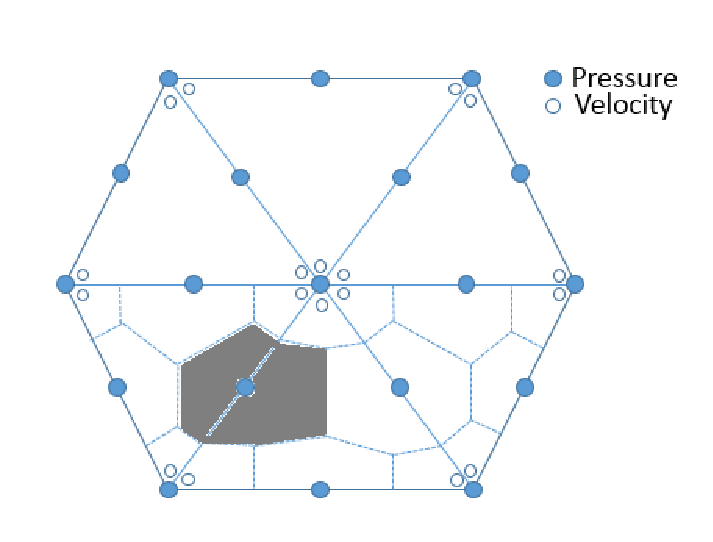
\includegraphics[width=.5\textwidth]{./Pics/P1DGP2.pdf}}
\caption{2D representation of \PN[1]{2} element pairs used in this work. Shaded areas denote control volumes across two contiguous elements. Blue and white circles represent pressure and velocity nodes, respectively.} 
\label{fig:fem_cv}
\end{figure}

\clearpage

%%%%
%%%%  FIGURE
%%%%
\begin{figure}[h]
\centering
\vbox{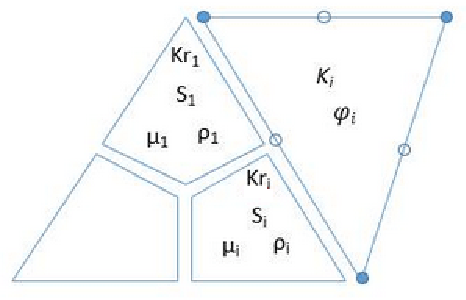
\includegraphics[width=.75\textwidth]{./Pics/element_n.pdf}}
\caption{This is a graphical representation of two different element types. Triangle {\it A} is a representation of the \PN[1]{2} element-pair, whereas triangle {\it B} represents the \PN[1]{1} element-pair. Porosity $\phi_{i}$, permeability {\bf K}$_{i}$, velocity and pressure are primarily represented in FE space whereas scalar fields (such as saturation, density, viscosity etc) are represented in CV space.}
\label{fig:fem_elem}
\end{figure}
\clearpage

%%%%
%%%%  FIGURE 
%%%%
\begin{figure}[h]
\centering
\vbox{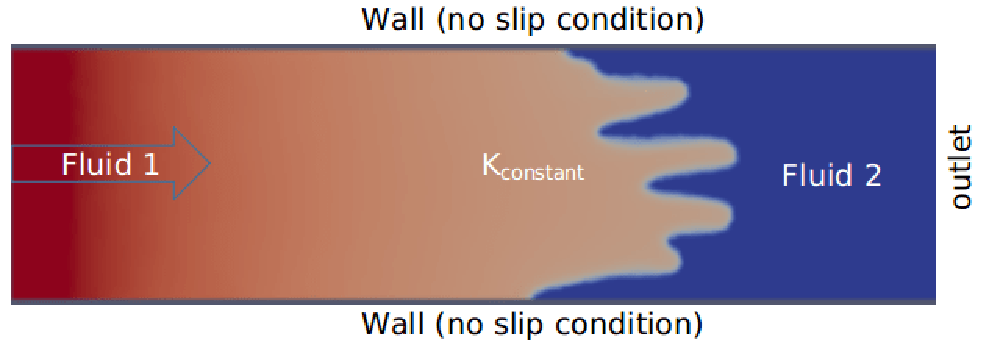
\includegraphics[width=0.75\textwidth]{./Pics/phase_vol_frac_uni_perm_1.pdf}}
\caption{Schematics of formation of flow instabilities during injection of a pure low viscosity fluid (red) into a domain saturated with a second fluid (dark blue). The ratio of viscosity between the two fluids is 5. In this case, the initially piston shape front collapses leading to the formation of several fingers.}
\label{fig:simple_case}
\end{figure}
\clearpage


%%%%
%%%%  FIGURE 
%%%%
\begin{figure}[ht] 
\vbox{
\hbox{\hspace{-0.3cm}
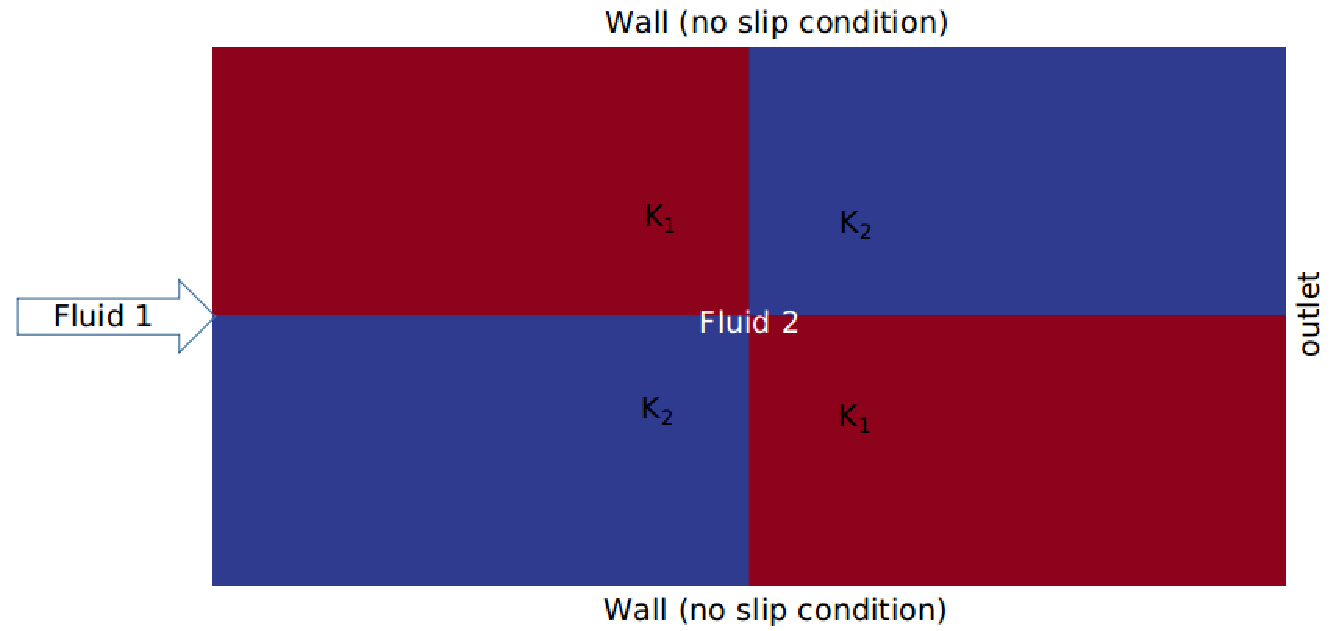
\includegraphics[width=.8\textwidth]{./Pics1/2b2_wi_fine/2b2_whole_in_fine_perm_1.pdf} 
}
\vspace{0.0cm}
\hbox{\hspace{3.5cm} (a) map of permeabilities ($\mathbf{K}$)
}
\vspace{0.25cm}
\hbox{\hspace{1.5cm}
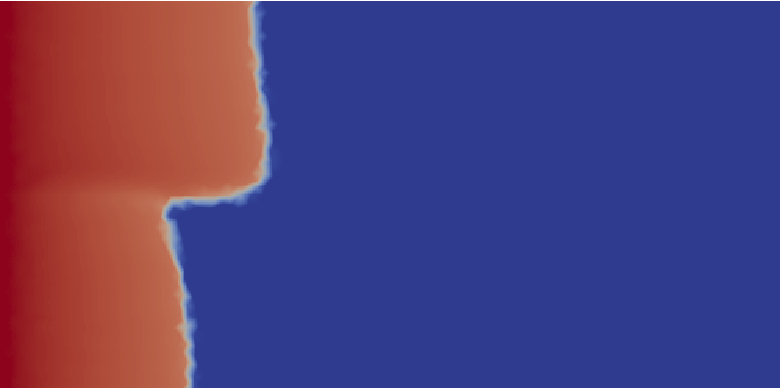
\includegraphics[width=.85\textwidth]{./Pics1/2b2_wi_fine/2b2_whole_in_fine_250_2.pdf}
}
\vspace{0.0cm}
\hbox{\hspace{4.5cm} (b) flow at t=250 
}
\vspace{0.25cm}
\hbox{\hspace{1.5cm}
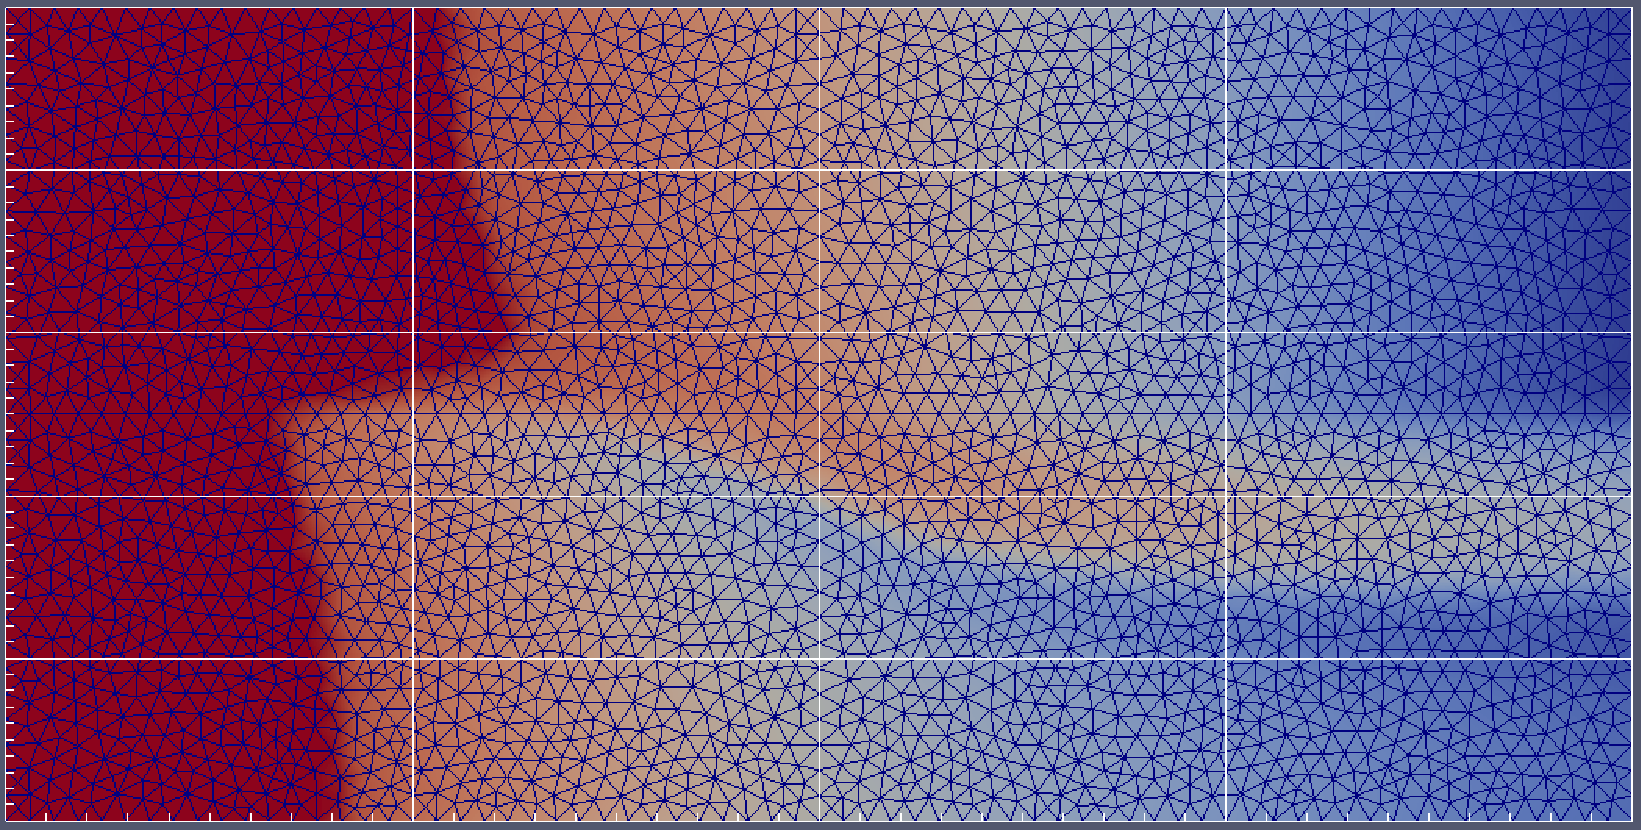
\includegraphics[width=.65\textwidth]{./Pics1/2b2_wi_fine/2b2_whole_in_fine_3000_2.pdf}
}
\vspace{0.0cm}
\hbox{\hspace{4.0cm} (c) flow at t=3000   
}}     
\caption{Model validation of fluid displacement in heterogeneous porous media ({\it VR}=1): (a) the domain is divided into four subdomains with prescribed synthetic permeability, $\mathbf{K}_{1}=1$ and $\mathbf{K}_{2}=2.5$; (b-c) snapshots of saturation (displacing fluid) field at t=$25$s and t=$300$ sec. The domain is discretised with $5960$ \PN[1]{2} elements. }
\label{fem_cv_represent_a}
\end{figure}
\clearpage



%%%%
%%%%  FIGURE
%%%%
\begin{landscape}
\begin{figure}[ht] 
\vbox{\vspace{-1cm}
\hbox{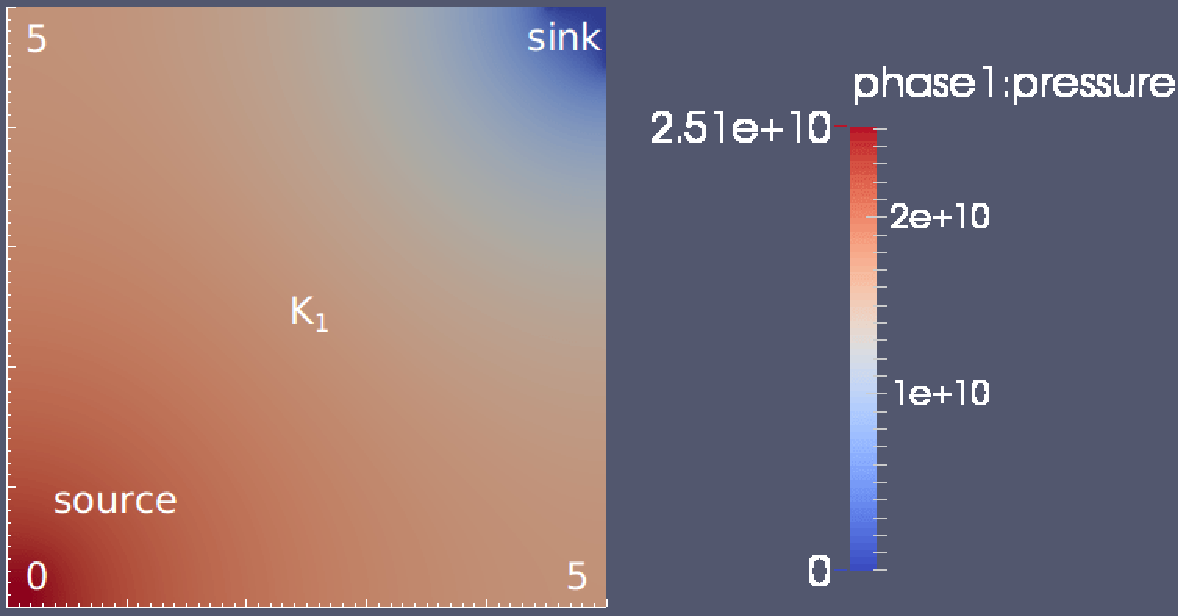
\includegraphics[width=.7\textwidth]{./Pics1/Saffman_homogeneous_MR3/saffman_homo_fixed_2.pdf}
      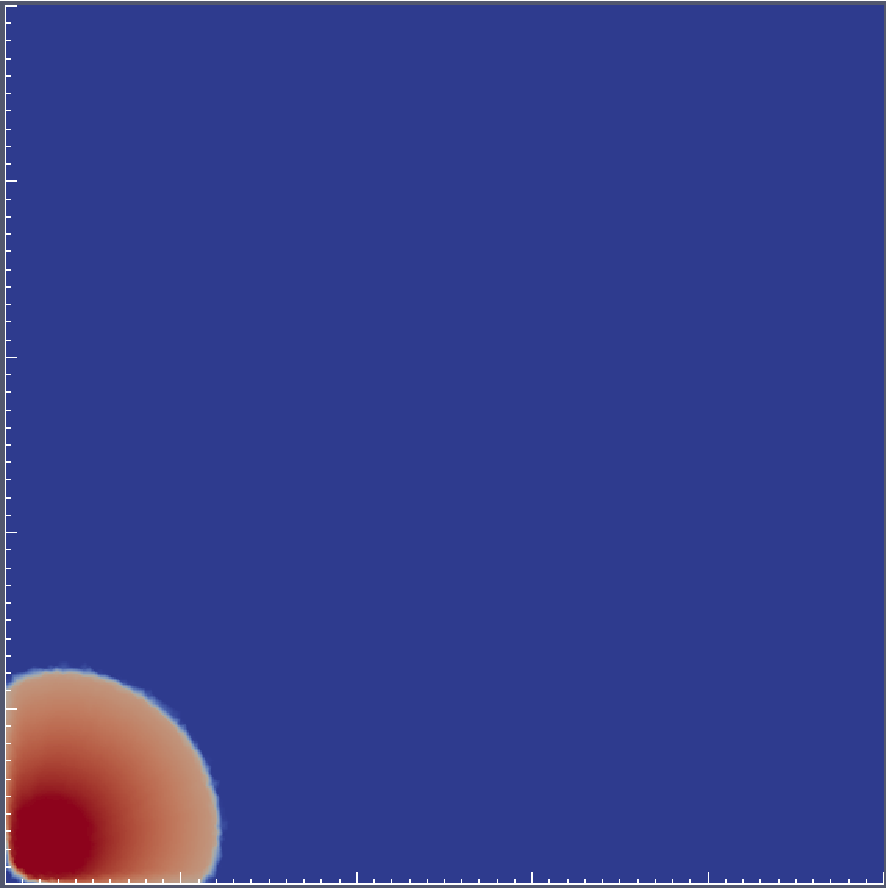
\includegraphics[width=.37\textwidth]{./Pics1/Saffman_homogeneous_MR3/saffman_homo_fixed_250.pdf}
      \includegraphics[width=.37\textwidth]{./Pics1/Saffman_homogeneous_MR3/saffman_homo_fixed_1000.pdf}}
\vspace{0.cm}
\hbox{\hspace{2.5cm} (a) pressure at t=0s \hspace{5.cm} (b) t=0.87s \hspace{2.75cm} (c) t=3.54s}
\vspace{0.5cm}
\hbox{
      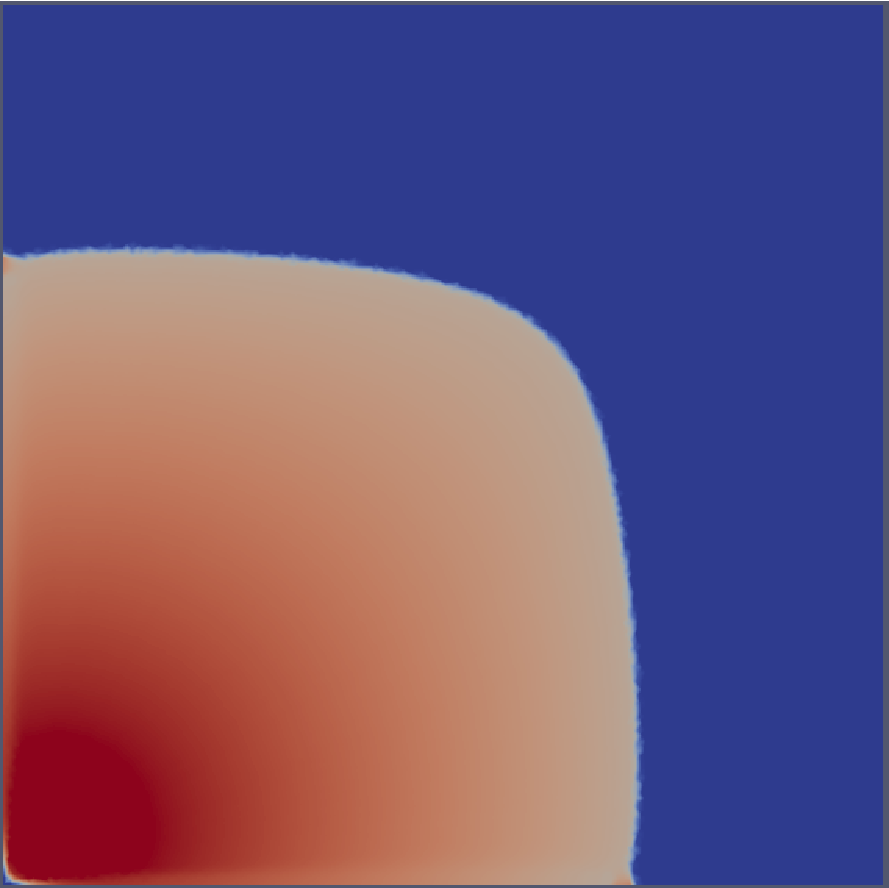
\includegraphics[width=.375\textwidth]{./Pics1/Saffman_homogeneous_MR3/saffman_homo_fixed_2500.pdf}
      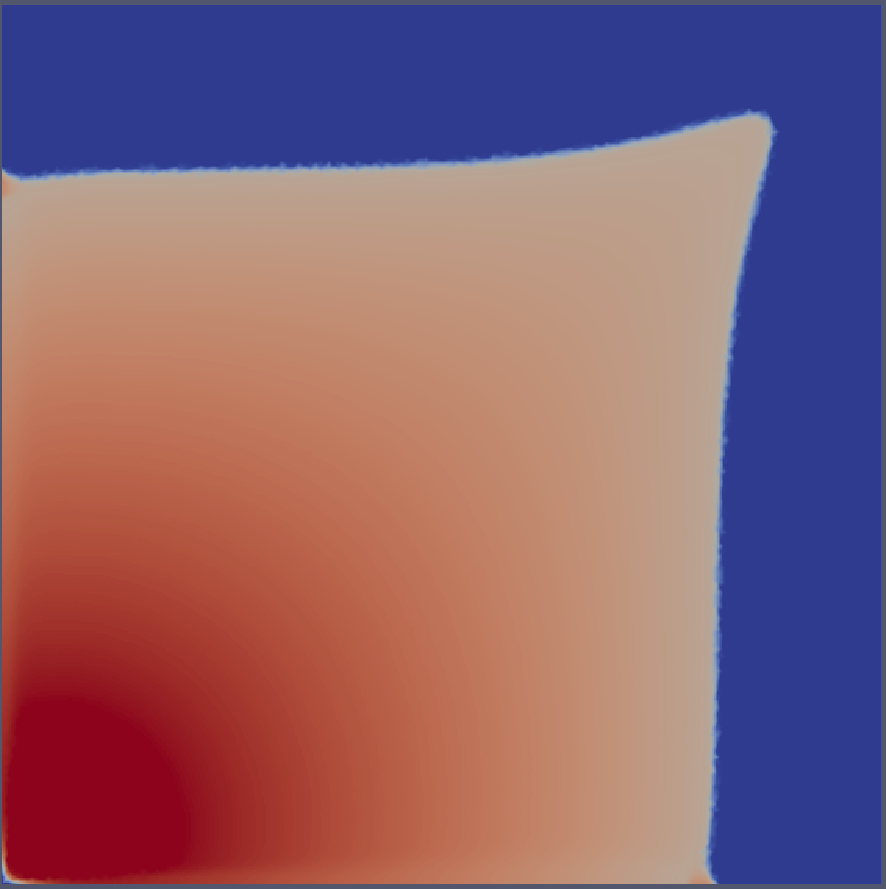
\includegraphics[width=.375\textwidth]{./Pics1/Saffman_homogeneous_MR3/saffman_homo_fixed_3500.pdf} 
      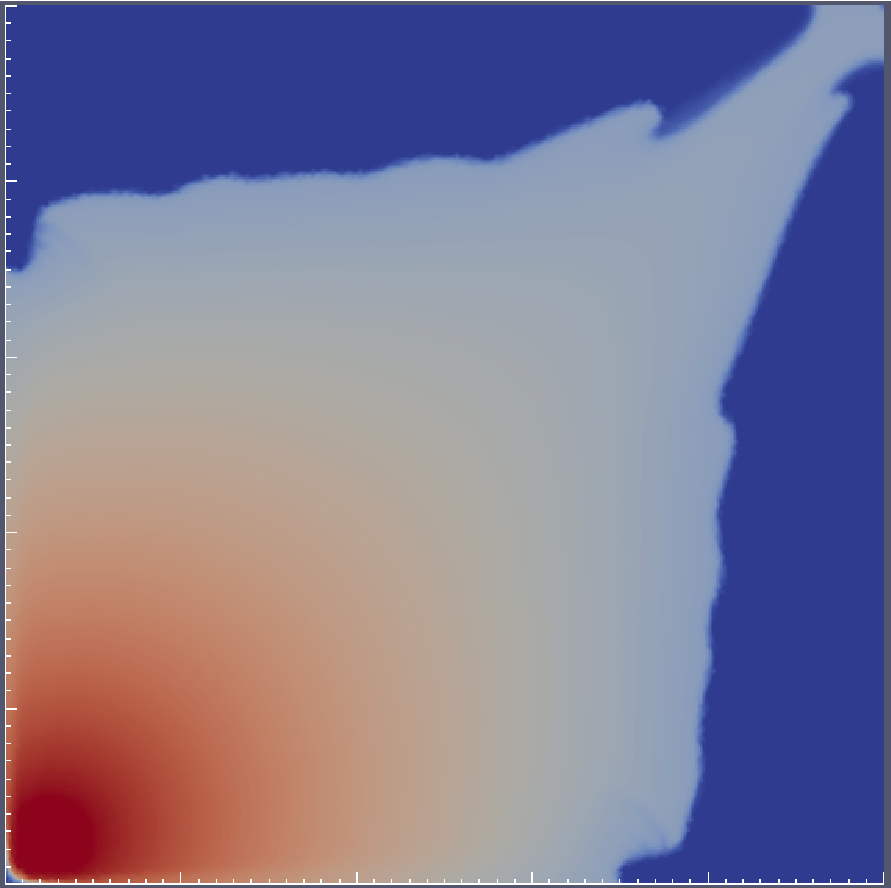
\includegraphics[width=.65\textwidth]{./Pics1/Saffman_homogeneous_MR3/saffman_homo_fixed_end.pdf}}
\vspace{0.cm}
\hbox{ \hspace{1.cm} (d) t=8.86s \hspace{3.0cm} (e) t=12.41s   \hspace{4.0cm} (f) t=17.95s}
\vspace{0.cm}
}   
\caption{Simulated flow in a Hele-Shaw cell ({\it VR}=3): (a) initial pressure profile $\left(\text{in g.cm}^{-1}\text{.s}^{-2}\right)$ with source and sink regions are explicitly shown along with dimensions (in cm); (b-f) snapshots of wetting phase saturation showing flow profile as the simulation evolves. The domain contains $47500$ \PN[1]{2} triangular elements.}
\label{fig:homoheleshaw_VN3}
\end{figure}
\end{landscape}
\clearpage



%%%%
%%%%  FIGURE
%%%%
\begin{landscape}
\begin{figure}[ht] 
\vbox{\vspace{-1cm}
\hbox{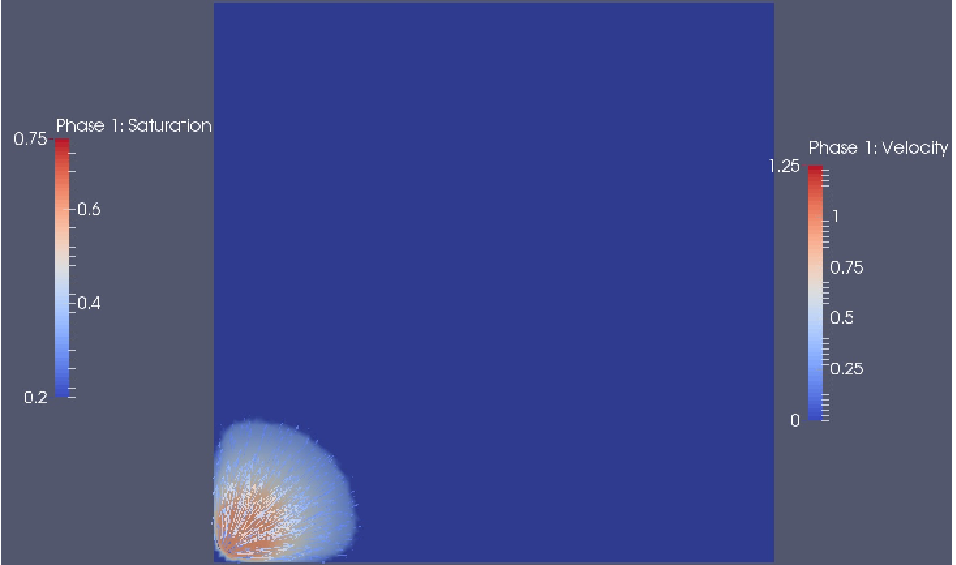
\includegraphics[width=.9\textwidth, height=0.5\textwidth]{./Pics1/Saffman_homogeneous_VR10/ST_Homog_VR10_D201c.pdf}
\hspace{0.5cm}      
      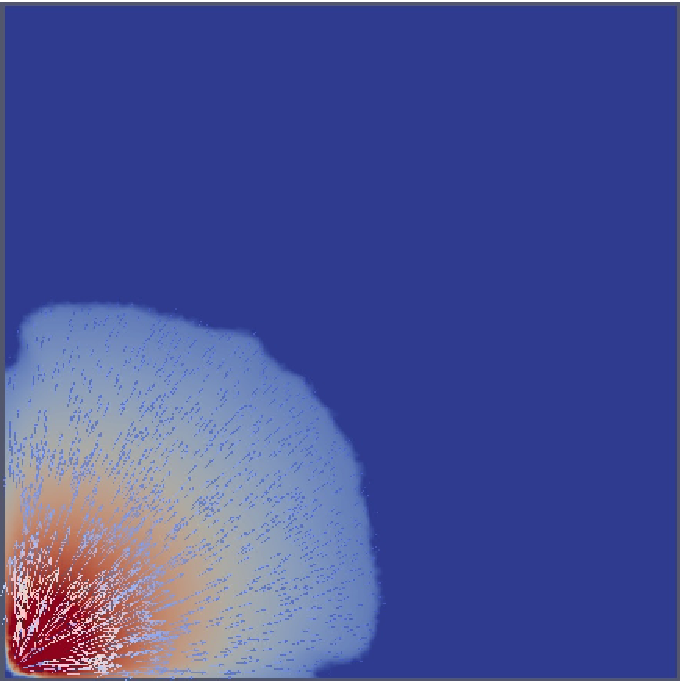
\includegraphics[width=.5\textwidth]{./Pics1/Saffman_homogeneous_VR10/ST_Homog_VR10_D1001c.pdf}}
\vspace{0.cm}
\hbox{\hspace{5.cm} (a) t=0.66s \hspace{8.cm} (b) t=3.43s }
\vspace{0.5cm}
\hbox{
      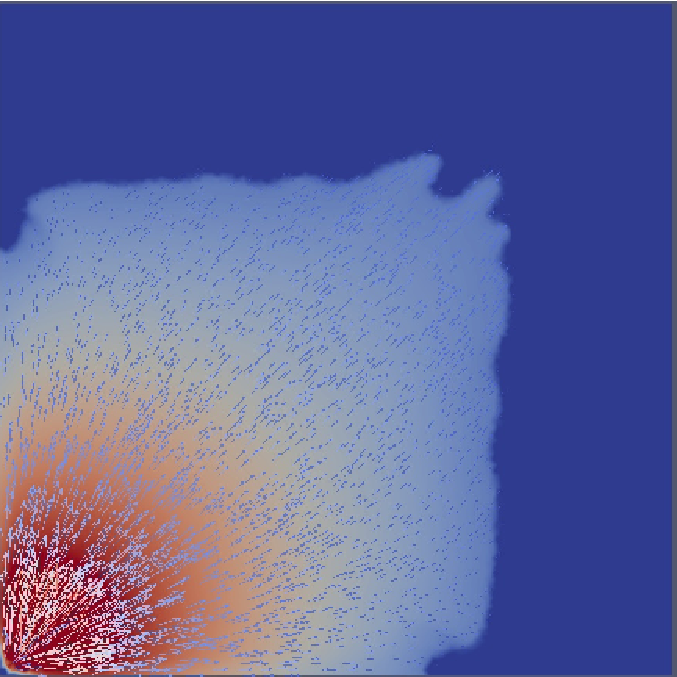
\includegraphics[width=.5\textwidth]{./Pics1/Saffman_homogeneous_VR10/ST_Homog_VR10_D2001c}
      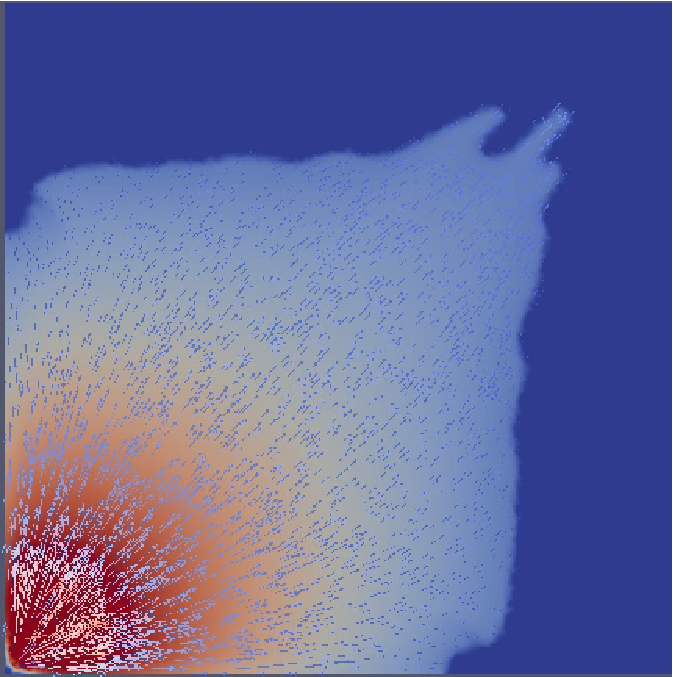
\includegraphics[width=.5\textwidth]{./Pics1/Saffman_homogeneous_VR10/ST_Homog_VR10_D2201c}
      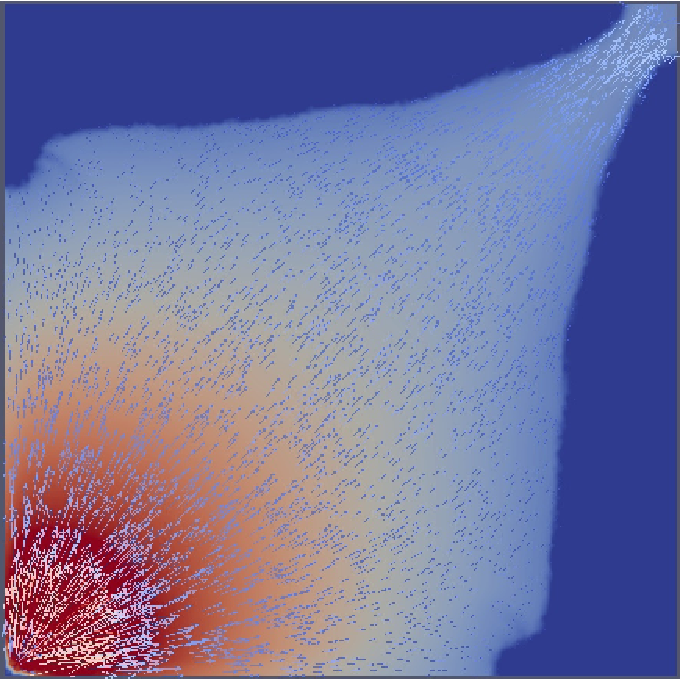
\includegraphics[width=.5\textwidth]{./Pics1/Saffman_homogeneous_VR10/ST_Homog_VR10_D3001c}}
\vspace{0.cm}
\hbox{ \hspace{2.cm} (c) t=6.92s \hspace{4.5cm} (d) t=7.61s \hspace{4.5cm} (e)t=10.00s}
\vspace{0.cm}
}   
\caption{Simulated flow in a Hele-Shaw cell ({\it VR}=10): snapshots of overlapped wetting phase saturation and velocity vectors showing flow profile as the simulation evolves. The domain contains $26313$ \PN[1]{2} triangular elements.}
\label{fig:homoheleshaw_VN10}
\end{figure}
\end{landscape}
\clearpage

%%%%
%%%%  FIGURE
%%%%
\begin{landscape}
\begin{figure}[ht] 
\vbox{\vspace{-1cm}
\hbox{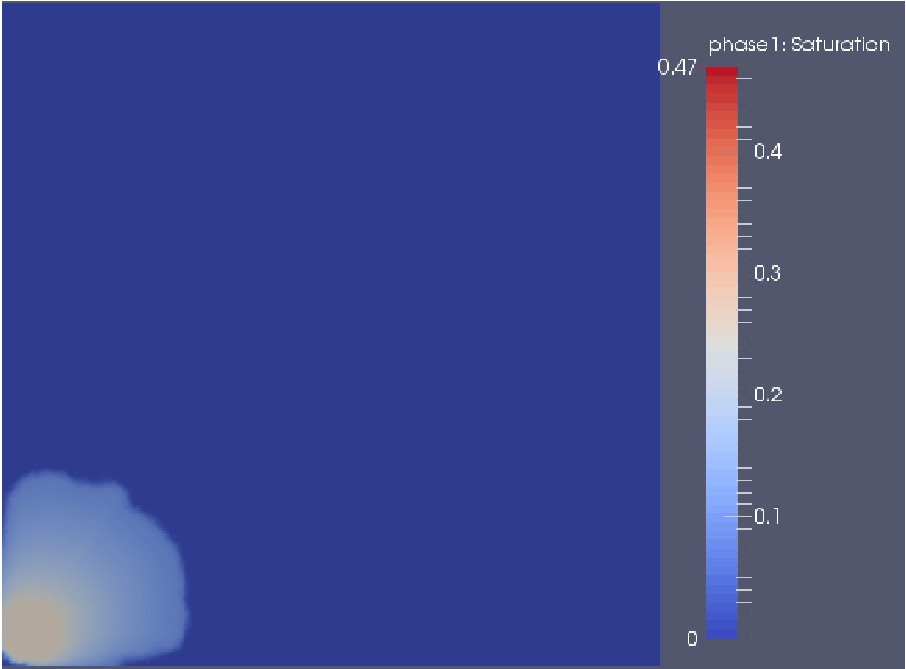
\includegraphics[width=.9\textwidth, height=0.5\textwidth]{./Pics1/Saffman_homogeneous_VR150/ST_Homog_VR150_D300b}
\hspace{0.5cm}      
      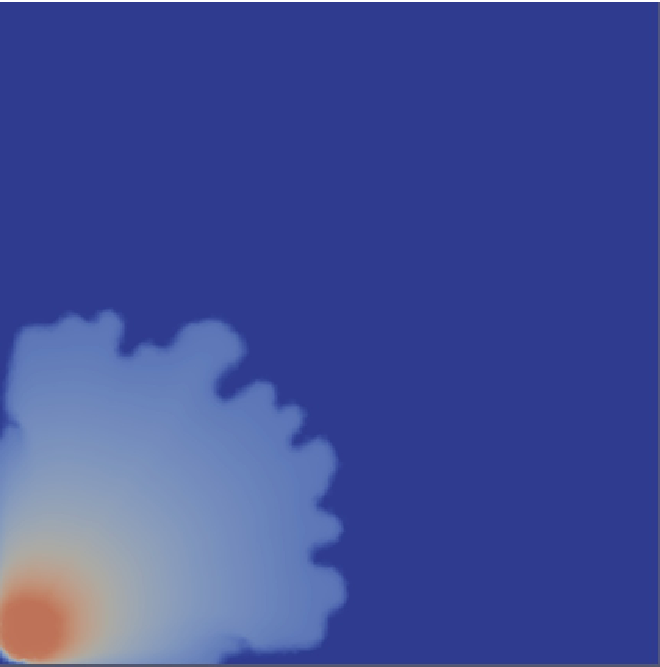
\includegraphics[width=.5\textwidth]{./Pics1/Saffman_homogeneous_VR150/ST_Homog_VR150_D1600b}}
\vspace{0.cm}
\hbox{\hspace{5.cm} (a) t=0.27s \hspace{8.cm} (b) t=0.94s }
\vspace{0.5cm}
\hbox{
      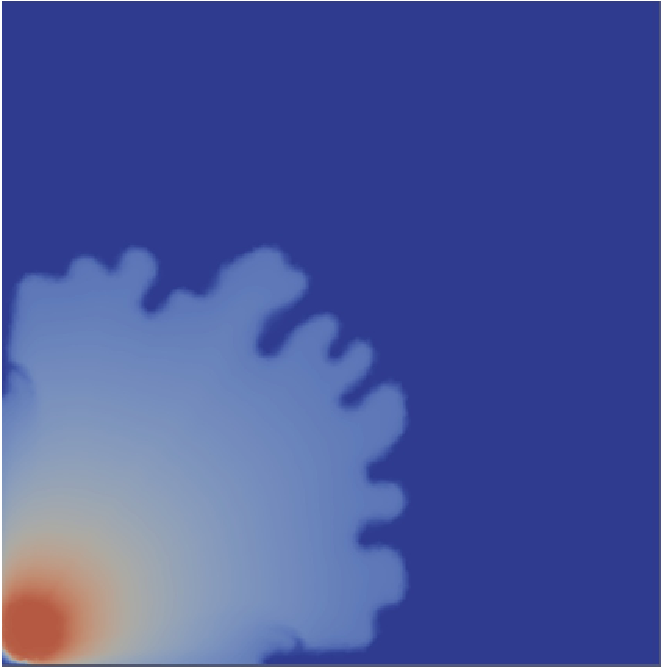
\includegraphics[width=.5\textwidth]{./Pics1/Saffman_homogeneous_VR150/ST_Homog_VR150_D2700b}
      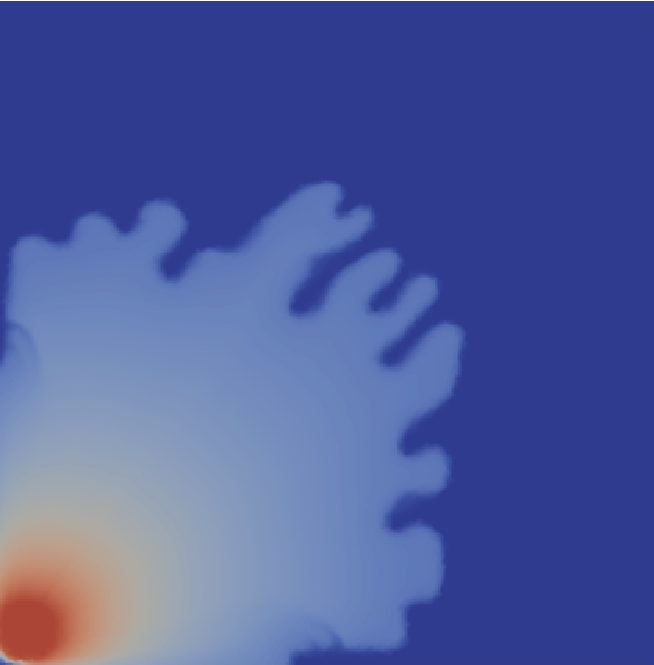
\includegraphics[width=.5\textwidth]{./Pics1/Saffman_homogeneous_VR150/ST_Homog_VR150_D4000b}
      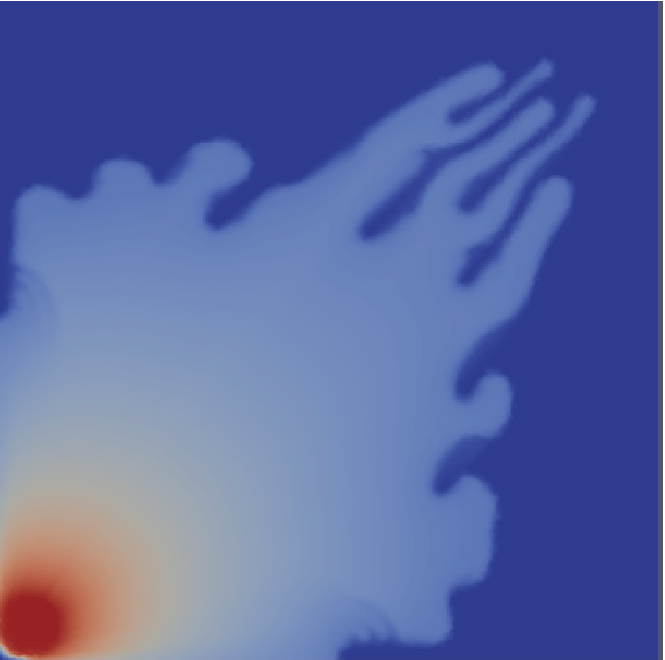
\includegraphics[width=.5\textwidth]{./Pics1/Saffman_homogeneous_VR150/ST_Homog_VR150_D7000b}}
\vspace{0.cm}
\hbox{ \hspace{2.cm} (c) t=1.32s \hspace{4.5cm} (d) t=1.70s \hspace{4.5cm} (e)t=2.31s}
\vspace{0.cm}
}   
\caption{Simulated flow in a Hele-Shaw cell ({\it VR}=150): snapshots of wetting phase saturation showing flow profile as the simulation evolves. The domain contains $26313$ \PN[1]{2} triangular elements.}
\label{fig:homoheleshaw_VN10}
\end{figure}
\end{landscape}
\clearpage


%%%%
%%%%  FIGURE
%%%%
\begin{landscape}
\begin{figure}[ht] 
\hbox{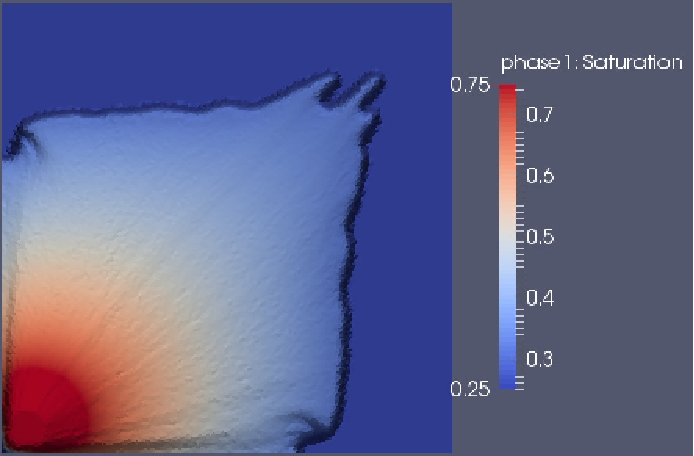
\includegraphics[width=.5\textwidth]{./Pics1/Saffman_homogeneous_VR10/ST_Homog_VR10_D2201_bbd}
       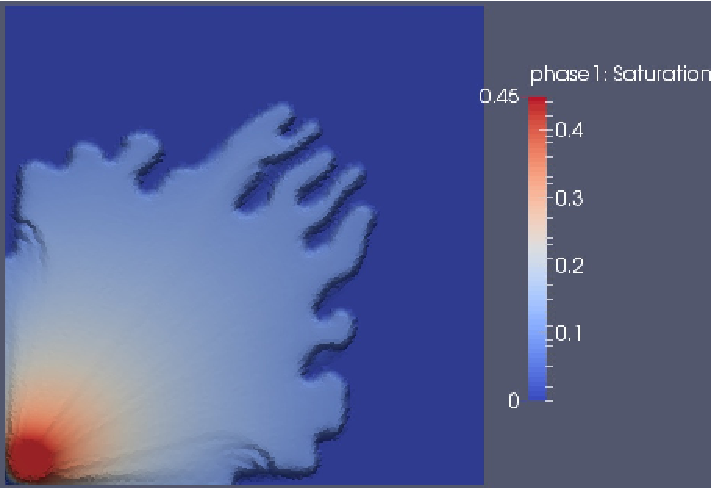
\includegraphics[width=.49\textwidth]{./Pics1/Saffman_homogeneous_VR150/ST_Homog_VR150_D5003_k2b}}
\caption{Simulated flow in Hele-Shaw cells performed with viscosity ratios of 10 (left, t=7.61s) and 150 (t=1.94s). Width of largest fingers are approximetely 0.70 and 0.90cm, which are in good agreement with values obtained from \citet{guan_2003}'s analytic solution. Domains of both simulations contain $26313$ \PN[1]{2} triangular elements.\red{(More pics to be added!!)}}
\label{fig:homoheleshaw_VN10_VN150}
\end{figure}
\end{landscape}



\begin{comment}

%%%%
%%%%  FIGURE
%%%%
\begin{landscape}
\begin{figure}[ht] 
\vbox{\vspace{-1cm}
\hbox{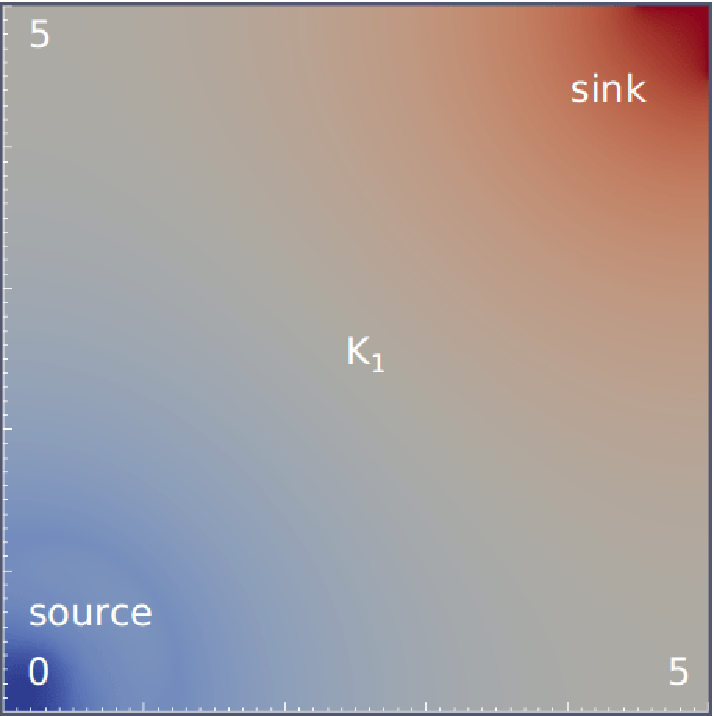
\includegraphics[width=.5\textwidth]{./Pics1/Saffman_homogeneous/saffman_homo_fixed_1.pdf}
      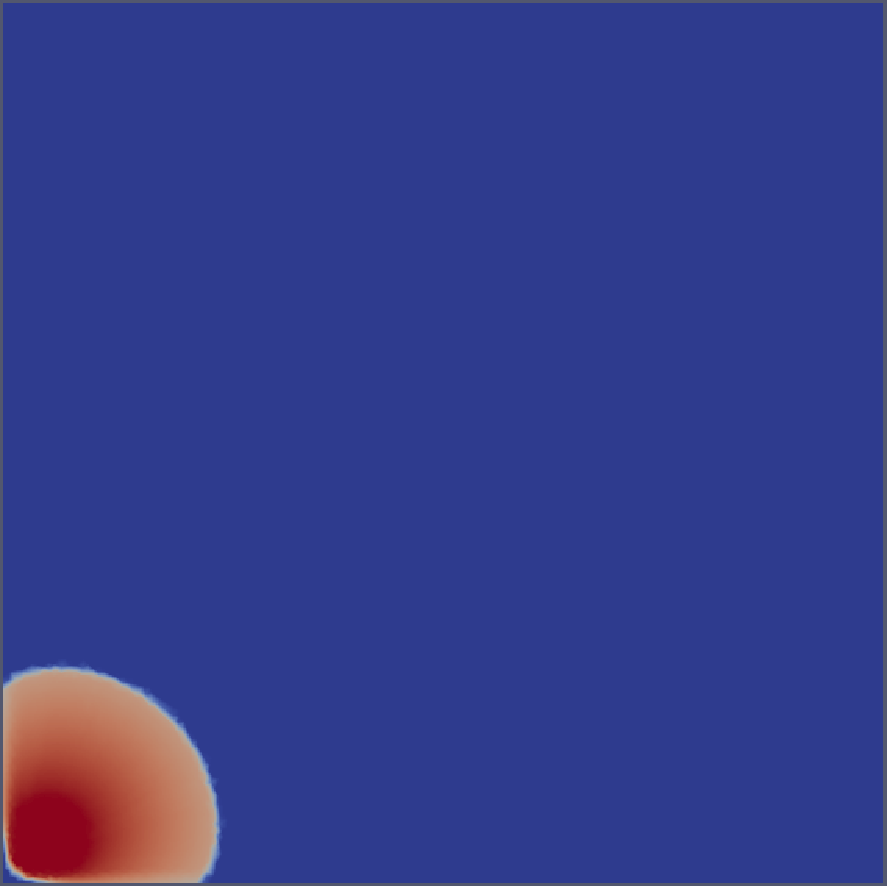
\includegraphics[width=.5\textwidth]{./Pics1/Saffman_homogeneous/saffman_homo_fixed_250_1.pdf}
      \includegraphics[width=.5\textwidth]{./Pics1/Saffman_homogeneous/saffman_homo_fixed_1000.pdf}}
\vspace{0.cm}
\hbox{\hspace{1.0cm} (a) pressure at t=0 \hspace{3.cm} (b) t=250\red{(???)} \hspace{3.0cm} (c) t=1000\red{(???)}}
\vspace{0.5cm}
\hbox{
      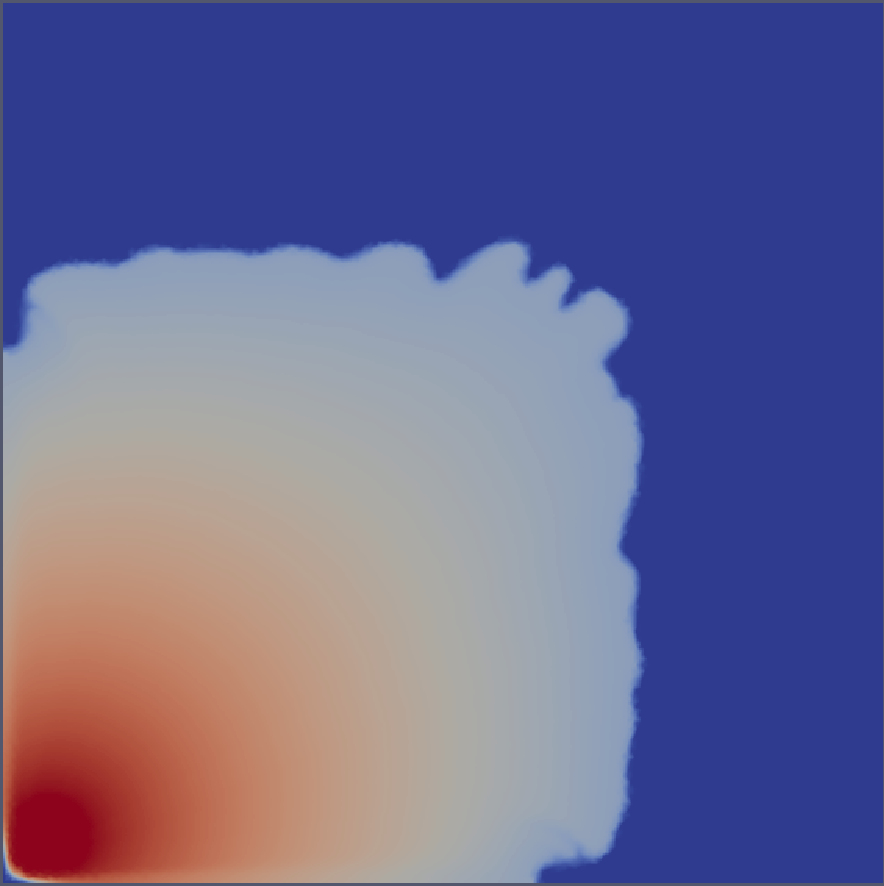
\includegraphics[width=.5\textwidth]{./Pics1/Saffman_homogeneous/saffman_homo_fixed_6000.pdf}
      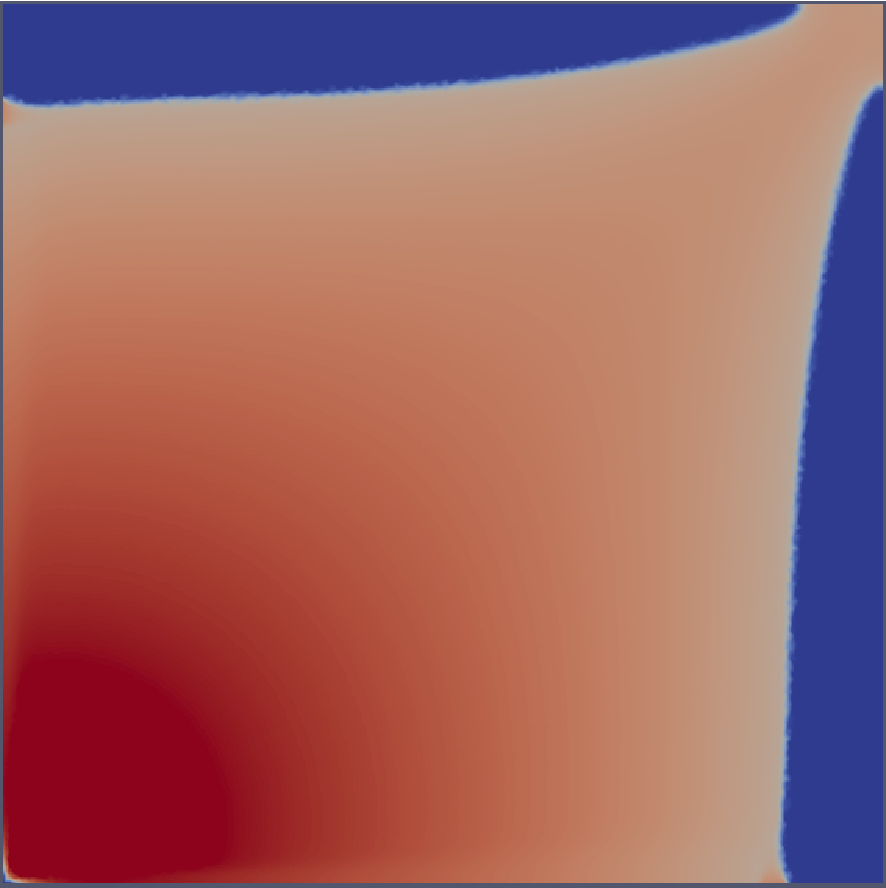
\includegraphics[width=.5\textwidth]{./Pics1/Saffman_homogeneous/saffman_homo_fixed_end_1.pdf}}
\vspace{0.cm}
\hbox{ \hspace{2.cm} (d) t=6000\red{(???)} \hspace{3.cm} (e) t=XXX\red{(???)}}
\vspace{0.cm}
}   
\caption{Simulated flow in a Hele-Shaw cell ({\it VR}=10): (a) pressure profile $\left(\text{in g.cm}^{-1}\text{.s}^{-2}\right)$ with source and sink regions explicitly shown along with dimensions (in cm); (b-e) snapshots of wetting phase saturation showing flow profile as the simulation evolves. The domain contains $47000$ \PN[1]{2} triangular elements. The pressure and saturation range of values are the same like the  case in fig.\ref{fig:homoheleshaw_VN3}.}
\label{fig:homoheleshaw_VN10}
\end{figure}
\end{landscape}
\clearpage
\end{comment}


%%%
%%% FIGURE XXXXXX
%%%
\begin{landscape}
  \begin{figure}[ht]
  \vbox{\vspace{-1cm}
      \hbox{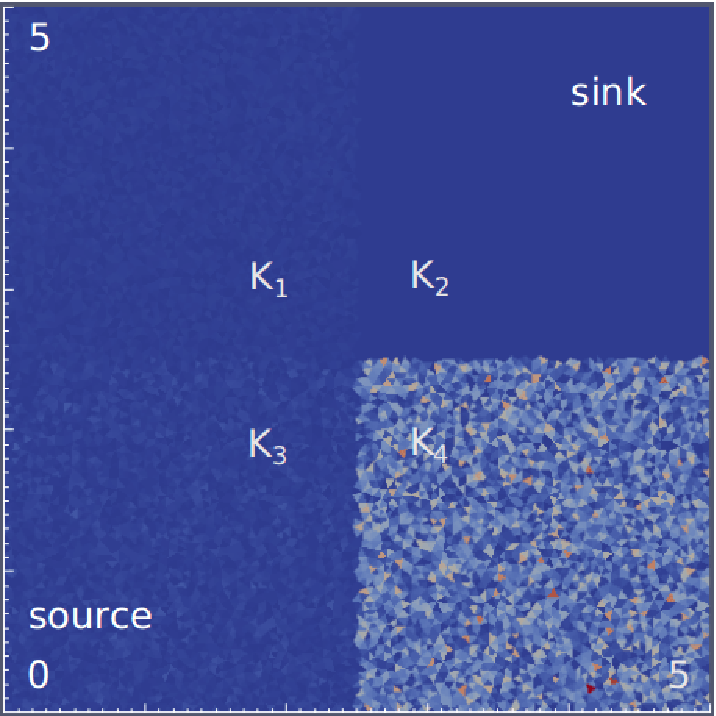
\includegraphics[width=.5\textwidth]{./Pics1/Saffman_heterogeneous/saffman_heter_fixed_1.pdf}
            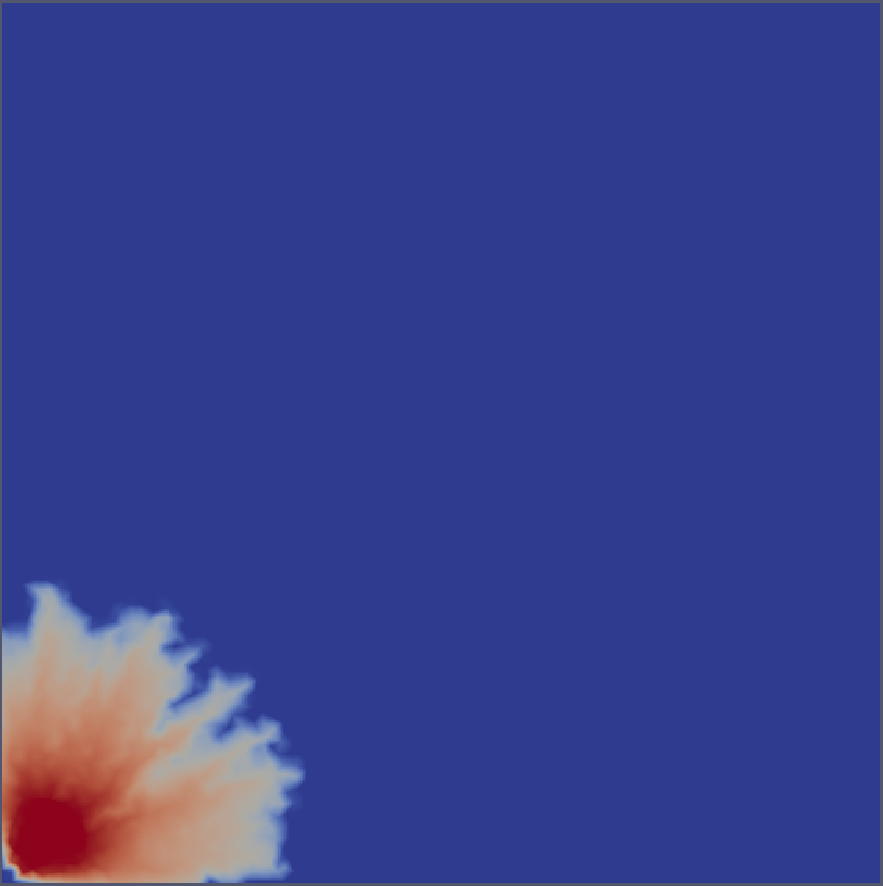
\includegraphics[width=.5\textwidth]{./Pics1/Saffman_heterogeneous/saffman_heter_fixed_500.pdf} 
            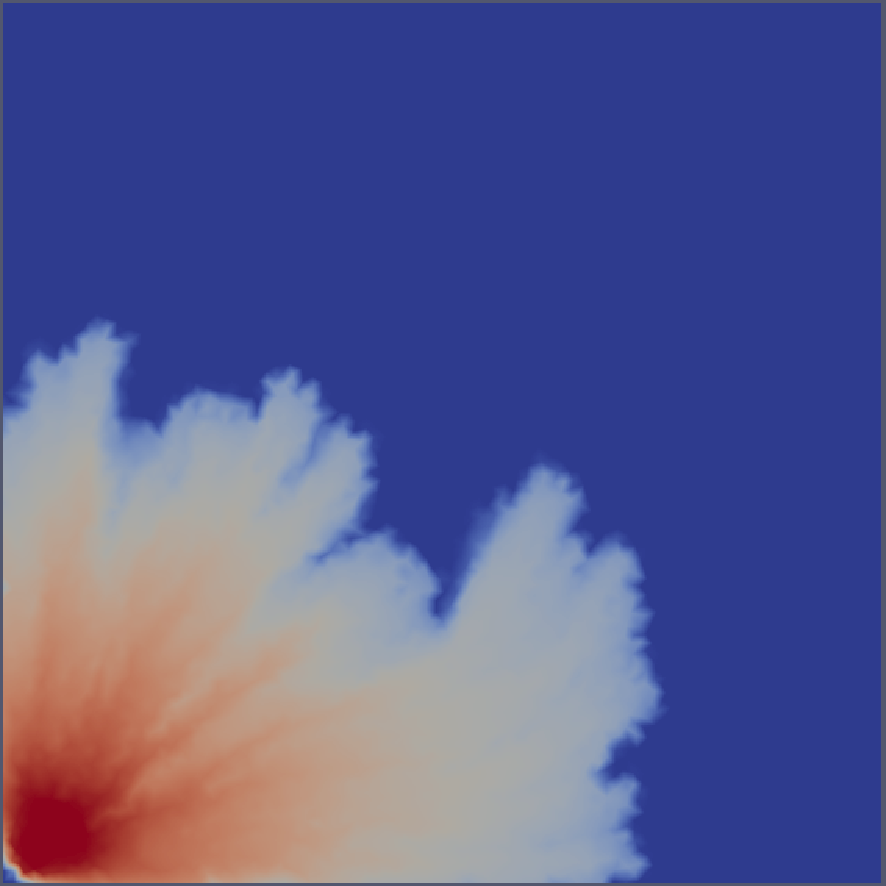
\includegraphics[width=.5\textwidth]{./Pics1/Saffman_heterogeneous/saffman_heter_fixed_2000.pdf} }
      \hbox{\hspace{1.0cm} (a) permeability map \hspace{3.cm} (b) t=0.75s \hspace{4.0cm} (c) t=8s}
      \vspace{0.5cm}
      \hbox{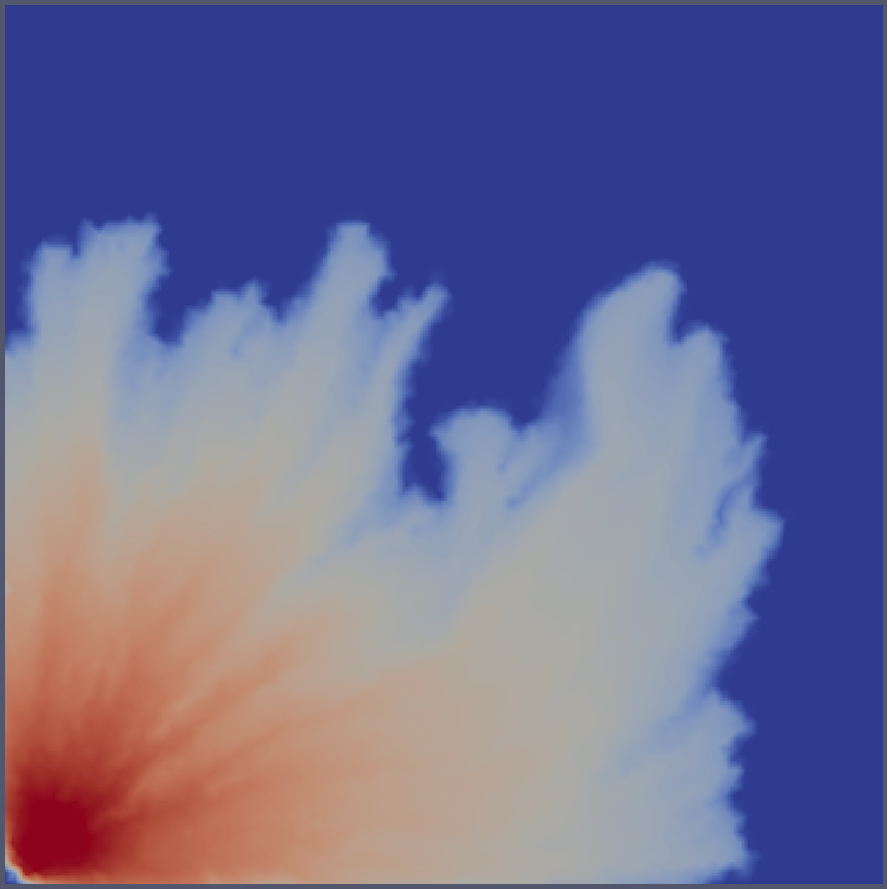
\includegraphics[width=.5\textwidth]{./Pics1/Saffman_heterogeneous/saffman_heter_fixed_3000.pdf}
            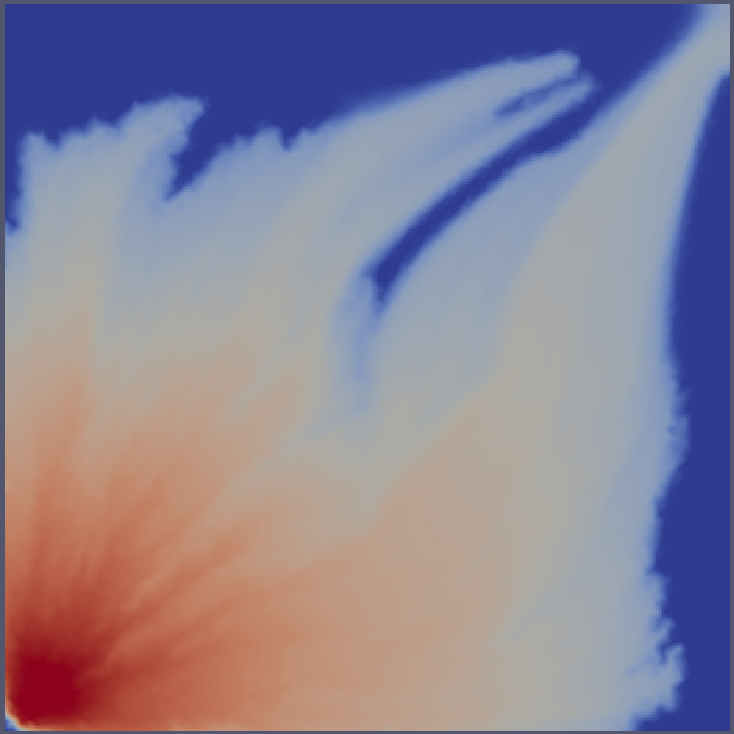
\includegraphics[width=.5\textwidth]{./Pics1/Saffman_heterogeneous/saffman_heter_fixed_6000.pdf}
            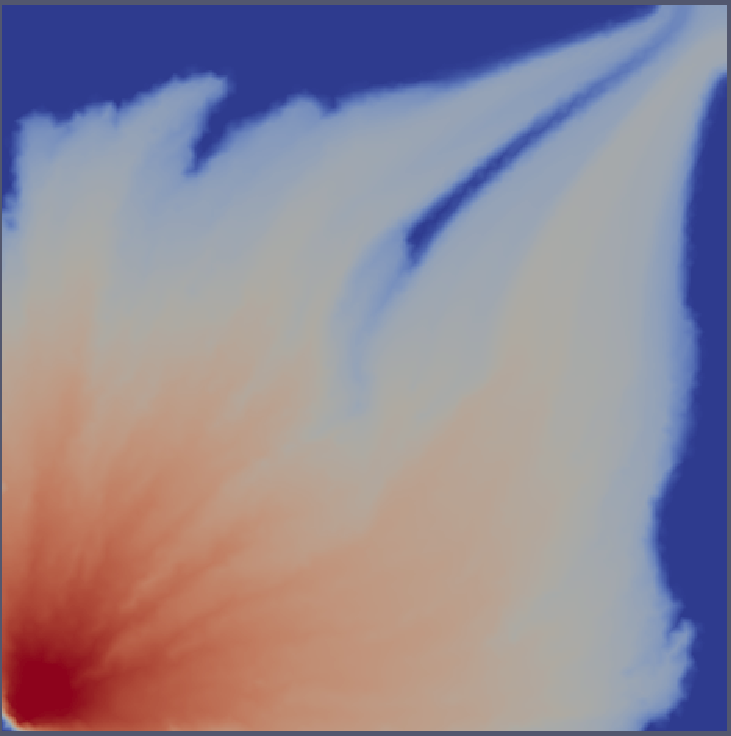
\includegraphics[width=.5\textwidth]{./Pics1/Saffman_heterogeneous/saffman_heter_fixed_24000.pdf} }
      \hbox{\hspace{2.5cm} (d) t=18s \hspace{5.cm} (e) t= \hspace{3.0cm} (f) t=24000 }}
\caption{Simulated flow in a modified Hele-Shaw cell with {\it VR}=10: (a) permeability distribution $\left(\text{10}^{-10}\le\mathbf{K}_{1}\le\text{5}\times\text{10}^{-10}\right.$, {\bf K}$_{2}$=10$^{-10}$, 10$^{-11}\le\mathbf{K}_{3}\le$ 5$\times$10$^{-10}$ and 10$^{-12}\le\mathbf{K}_{4}\le$ 5$\times$10$\left.^{-10}\text{ cm}^{2}\right)$; (b-f) snapshots of saturation profile during \red{XX} seconds of simulation. The domain contains \red{XX} \PN[1]{2} element-pairs.}
\label{fig:HeleShawHeter_VR10}
\end{figure}
\end{landscape}
\clearpage



%%%%
%%%%  FIGURE
%%%%
\begin{landscape}
\begin{figure}[ht] 
\vbox{
\hbox{\hspace{4.0cm}
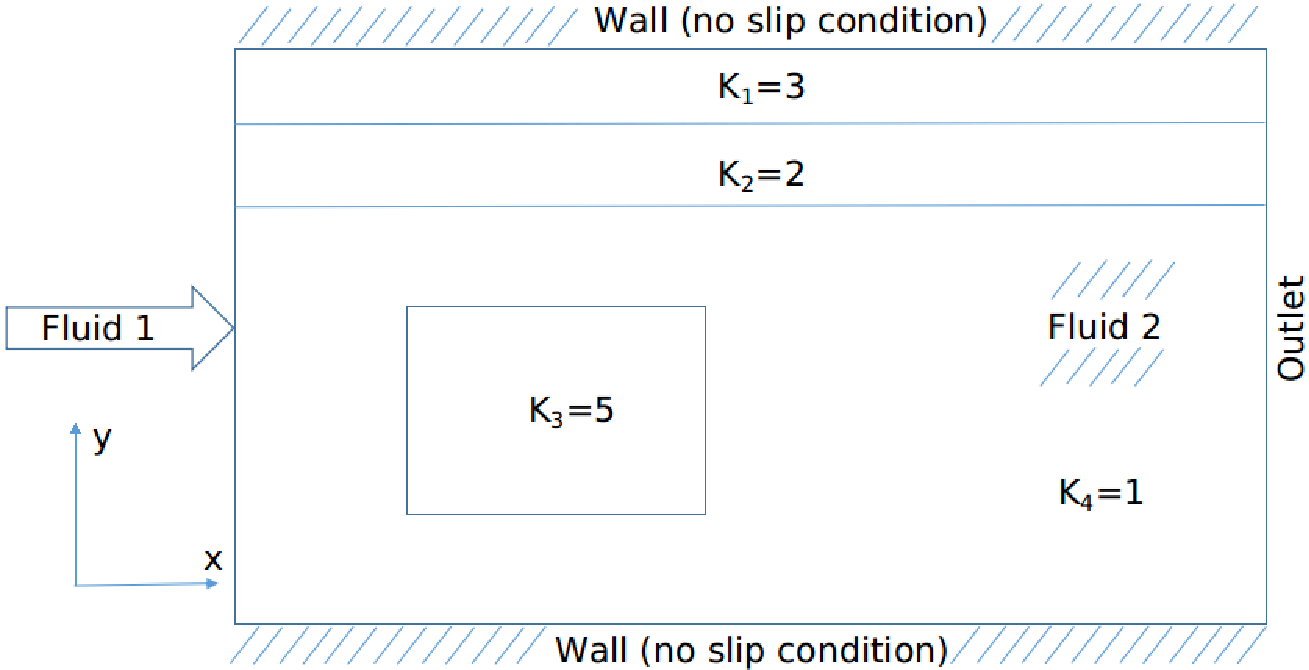
\includegraphics[width=.75\textwidth]{./Pics/map_of_boundaries.pdf} 
}
\vspace{0.0cm}
\hbox{\hspace{6.5cm} (a) map of permeabilties K   
}
\vspace{0.25cm}
\hbox{\hspace{4.0cm}
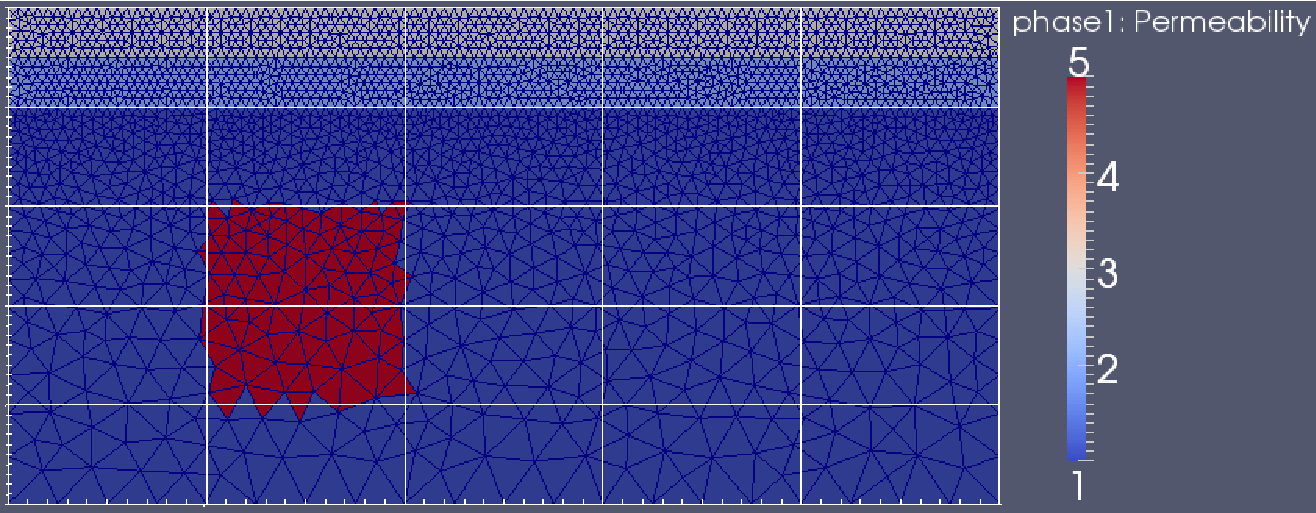
\includegraphics[width=.9\textwidth]{./Pics/map_of_boundaries_1.pdf}
}
\vspace{0.0cm}
\hbox{\hspace{9cm} (b)      
}
}     
\caption{Figure (a) describes the initial and boundary conditions as these are applied in this set of simulations. Below (b) there is a comparison between the unstructured and fixed mesh and the unstructured and adaptive mesh. During the implementation of fixed mesh initially there $4606$ elements while for the adaptive mesh there are $606$ while the majority of them is on the interface between between the two fluids. }
\label{fig:testcase_heter_domain}
\end{figure}
\end{landscape}
\clearpage



%%%%
%%%%  FIGURE
%%%%
\begin{landscape}
\begin{figure}[ht] 
\vbox{
\hbox{\hspace{3.5cm}
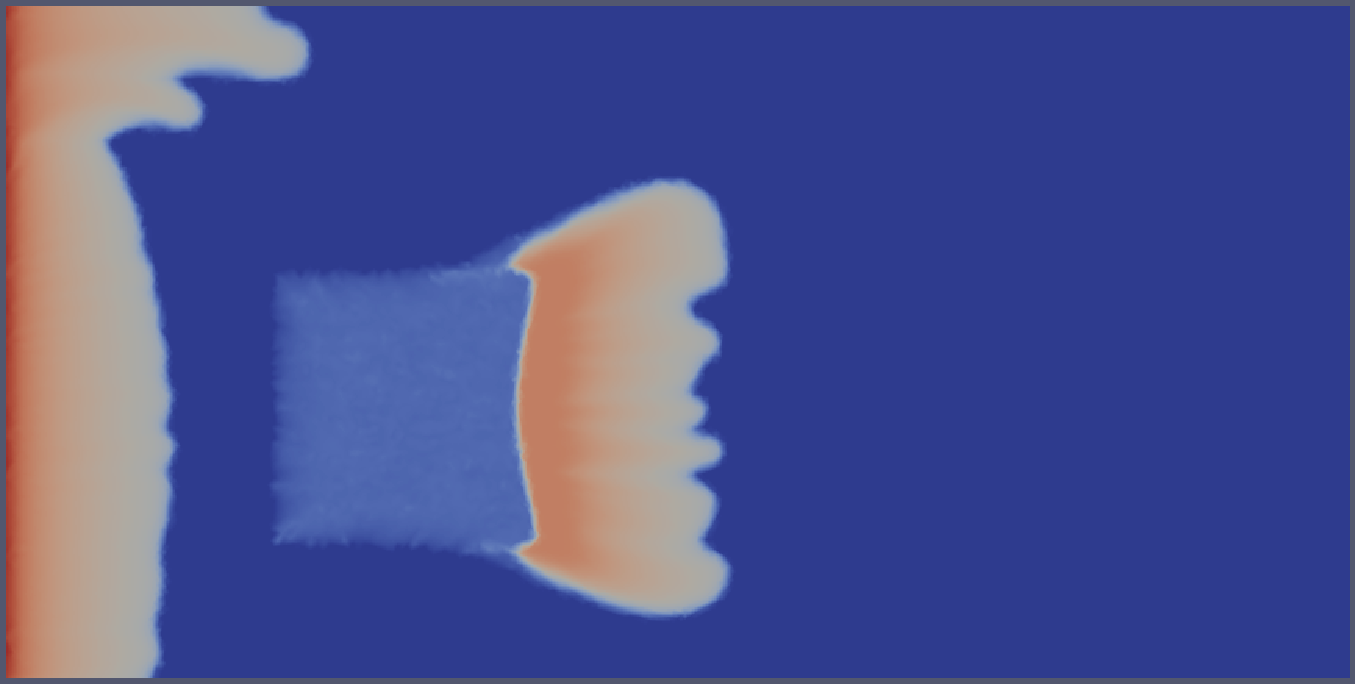
\includegraphics[width=.65\textwidth]{./Pics1/mr10_5regions_fixed/5regions_fixed_250.pdf} 
}
\vspace{0.0cm}
\hbox{\hspace{6.5cm} (a) flow at t=250 (fixed mesh)  
}
\vspace{0.25cm}
\hbox{\hspace{3.5cm}
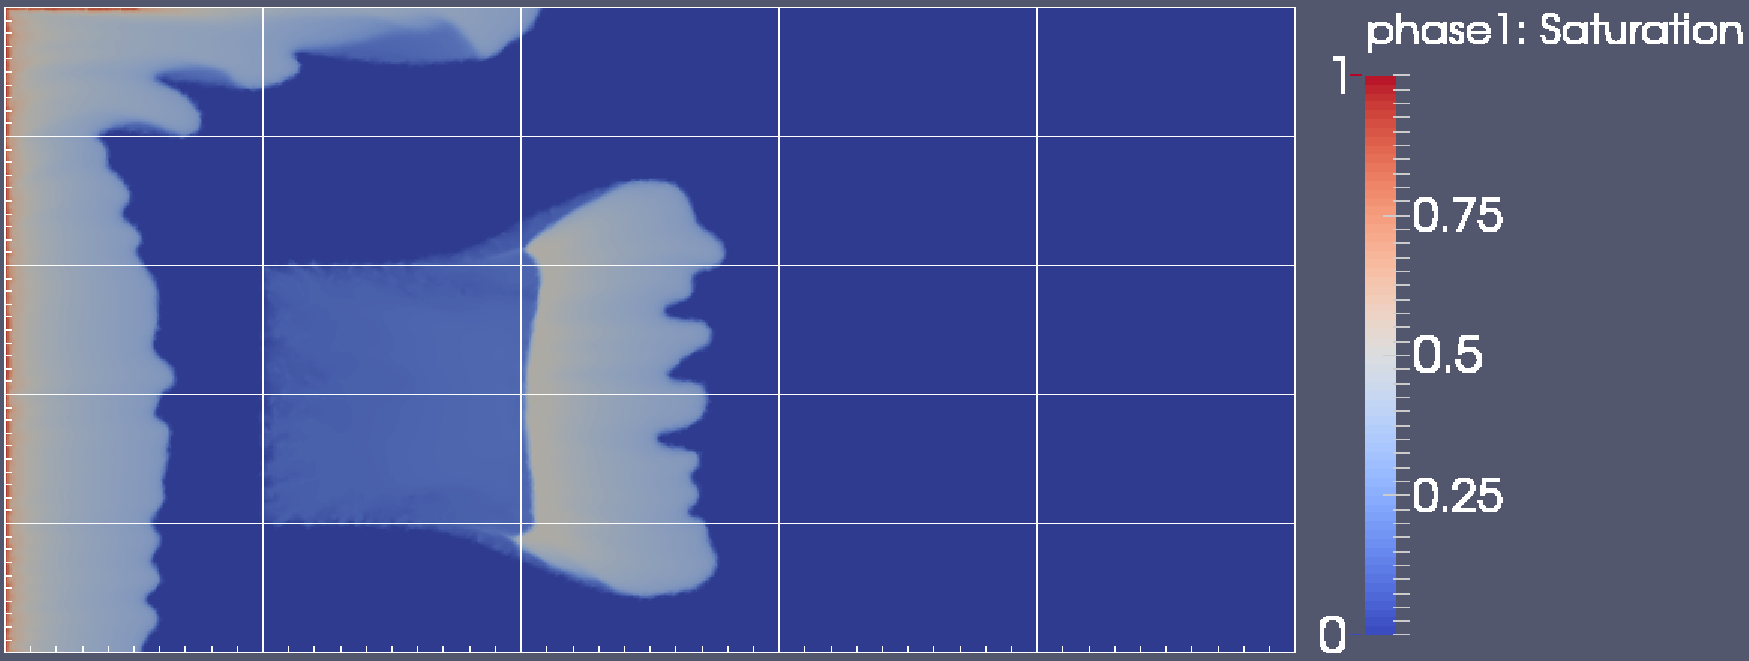
\includegraphics[width=.9\textwidth]{./Pics1/mr10_5regions_adapt/5regions_adapt_250_1.pdf}
}
\vspace{0.0cm}
\hbox{\hspace{6.5cm} (b) flow at t=250 (adaptive mesh)    
}
}     
\caption{For $t=0.125$s, $2$ test-cases under the VR=$10$ and under fixed (top) and adaptive(bottom) mesh are compared. There is a significant difference on the main front (left hand side of the domain) and the number of finger that appear.}
\label{fig:2testcase_a}
\end{figure}
\end{landscape}
\clearpage


%%%%
%%%%  FIGURE
%%%%
\begin{landscape}
\begin{figure}[ht] 
\vbox{
\hbox{\hspace{3.5cm}
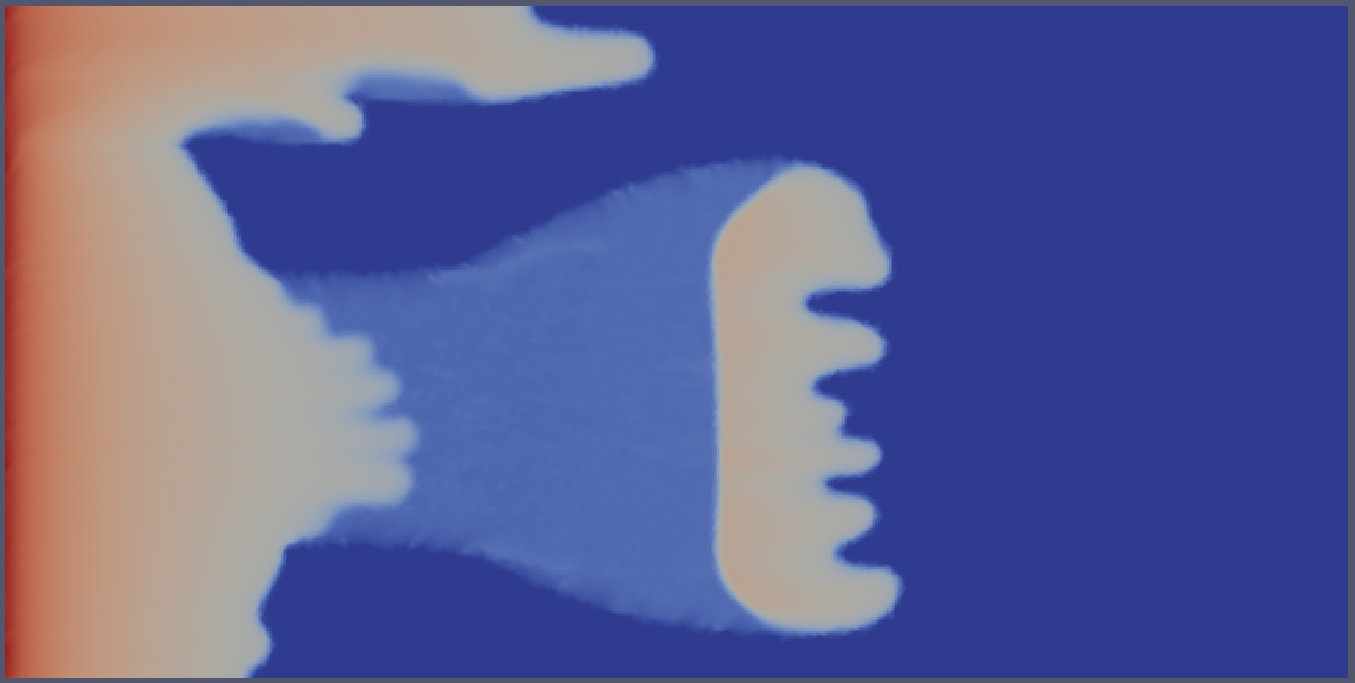
\includegraphics[width=.65\textwidth]{./Pics1/mr10_5regions_fixed/5regions_fixed_500.pdf} 
}
\vspace{0.0cm}
\hbox{\hspace{6.5cm} (a) flow at t=500 (fixed mesh)   
}
\vspace{0.25cm}
\hbox{\hspace{3.5cm}
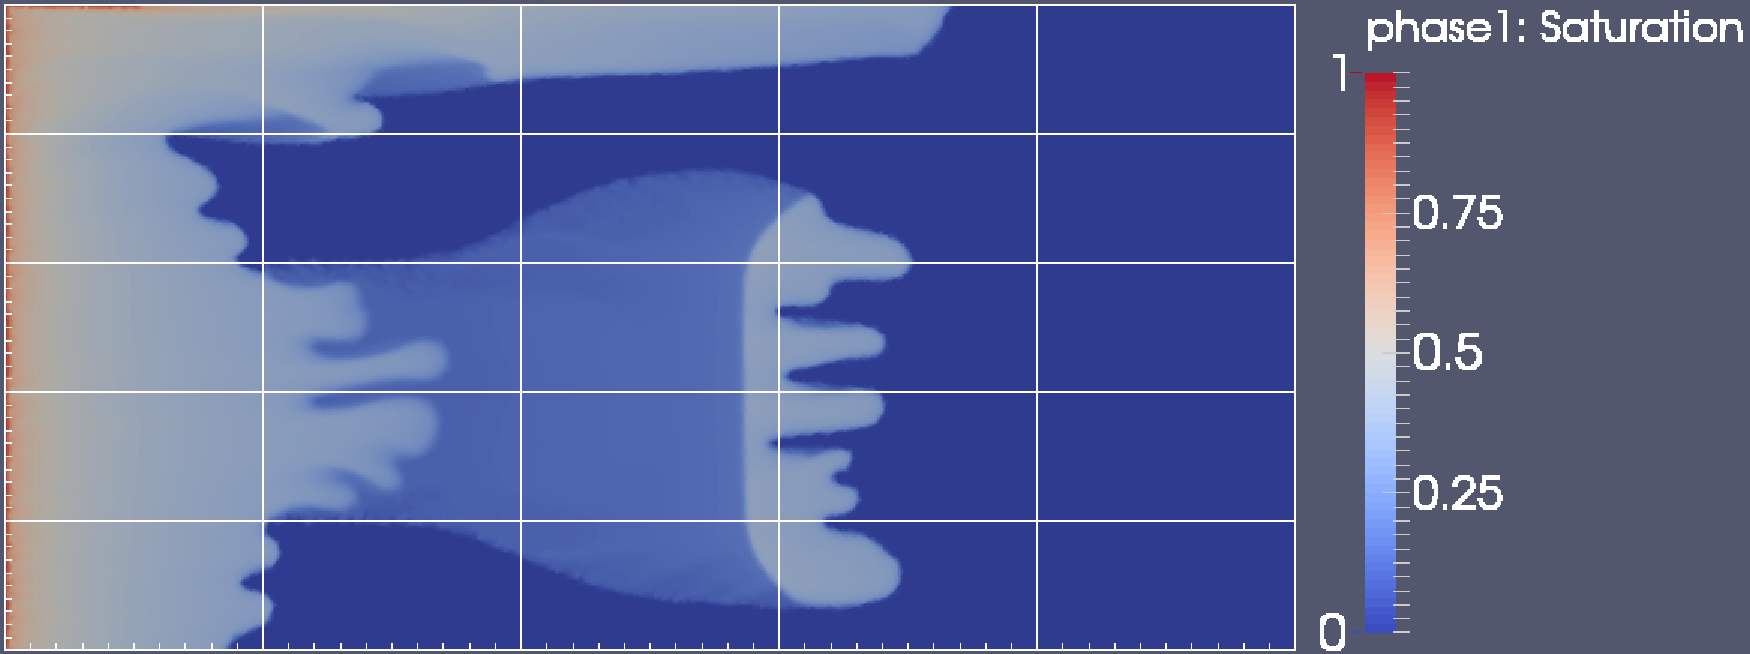
\includegraphics[width=.9\textwidth]{./Pics1/mr10_5regions_adapt/5regions_adapt_500_1.pdf}
}
\vspace{0.0cm}
\hbox{\hspace{6.5cm} (b) flow at t=500 (adaptive mesh)     
}
}     
\caption{At $t=0.25$s ($t=500$, timestemp) cross flow is taking place at the upper part of the formation. The fingers start to becoming more proufound as can been seen at the bottom.}
\label{fig:2testcase_b}
\end{figure}
\end{landscape}
\clearpage



%%%%
%%%%  FIGURE
%%%%
\begin{landscape}
\begin{figure}[ht] 
\vbox{
\hbox{\hspace{3.5cm}
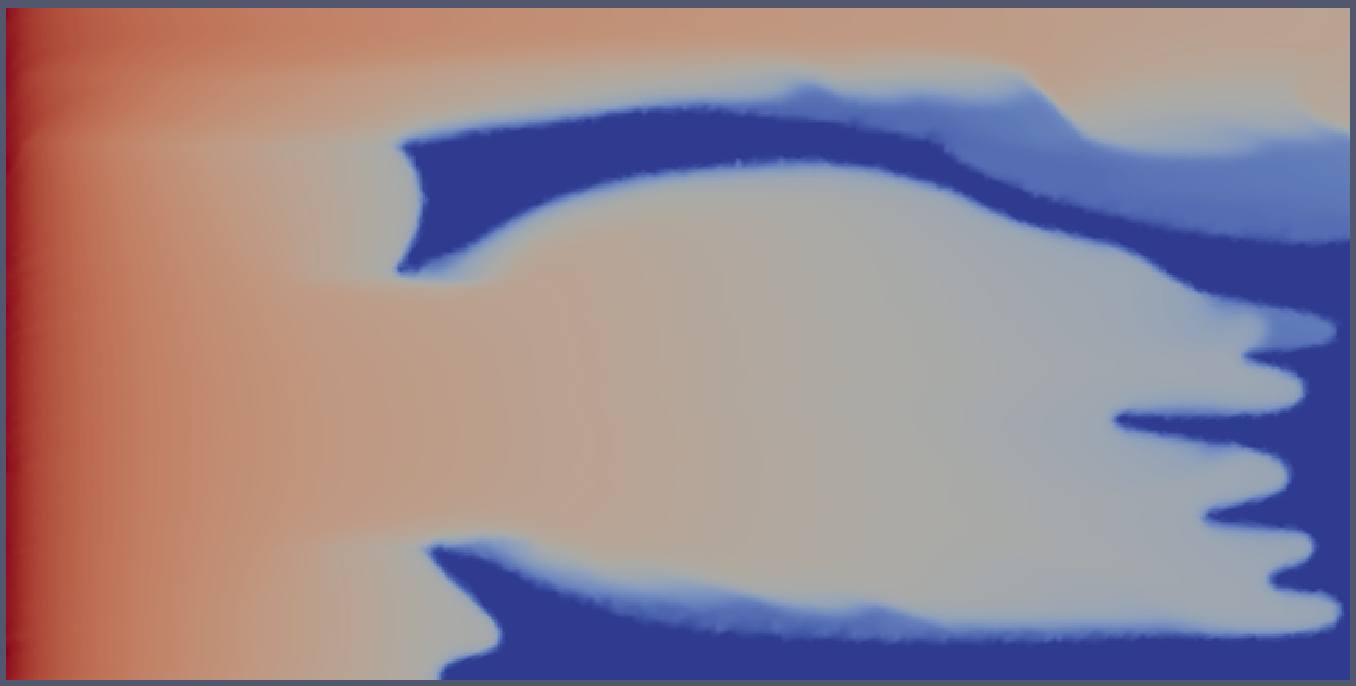
\includegraphics[width=.65\textwidth]{./Pics1/mr10_5regions_fixed/5regions_fixed_1500.pdf} 
}
\vspace{0.0cm}
\hbox{\hspace{6.5cm} (a) flow at t=1500 (fixed mesh)   
}
\vspace{0.25cm}
\hbox{\hspace{3.5cm}
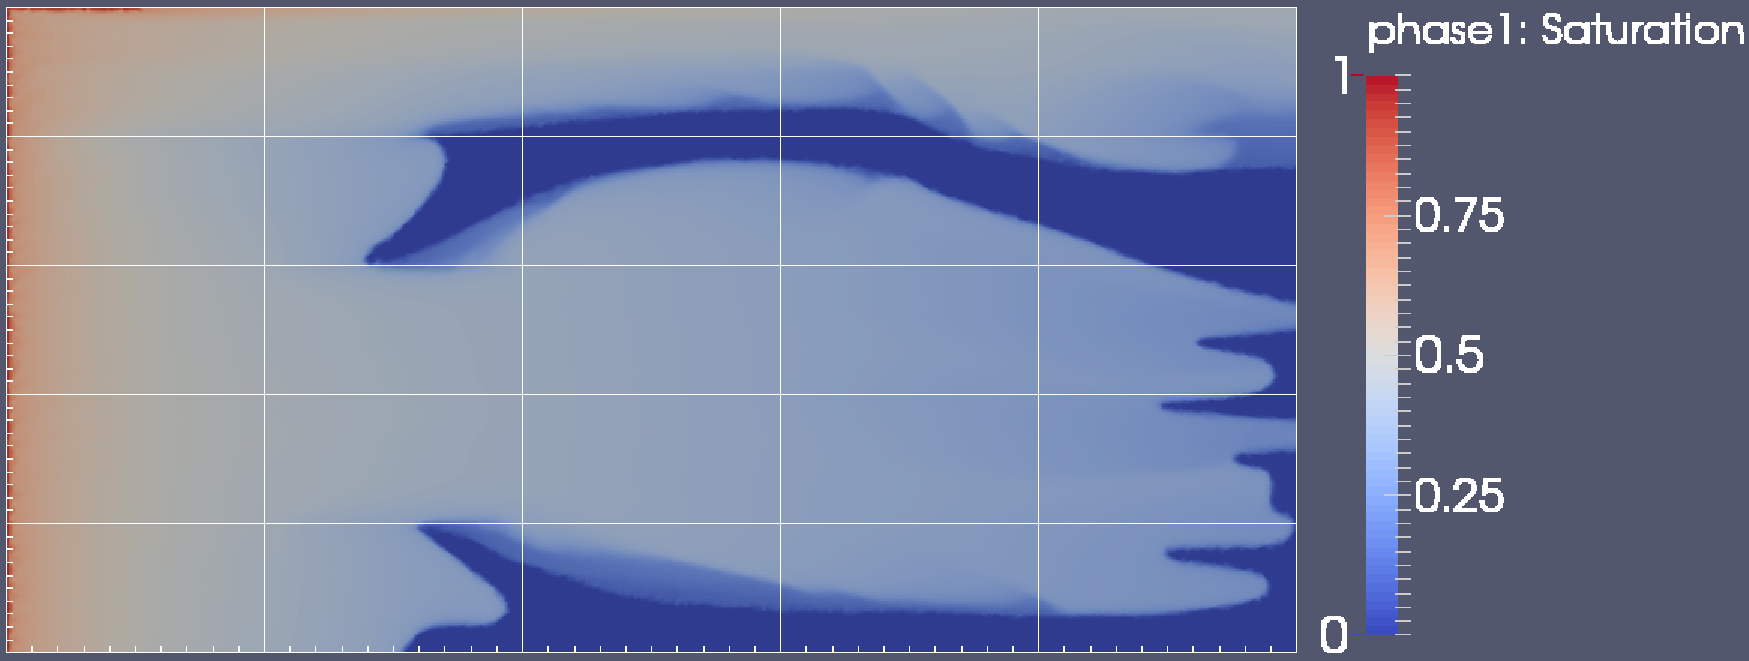
\includegraphics[width=.9\textwidth]{./Pics1/mr10_5regions_adapt/5regions_adapt_1500_1.pdf}
}
\vspace{0.0cm}
\hbox{\hspace{6.5cm} (b) flow at t=1500 (adaptive mesh)     
}
}     
\caption{At $t=0.75 sec$ ($t=1500$, timestemp) the initial cross flow is now fully developed and has travel all the way towards the outlet (right-hand side). and the finger below start forming a front that is also travelling towards the left-hand side.}
\label{fig:2testcase_c}
\end{figure}
\end{landscape}
\clearpage



%%%%
%%%%  FIGURE
%%%%
\begin{landscape}
\begin{figure}[ht] 
\vbox{
\hbox{\hspace{3.5cm}
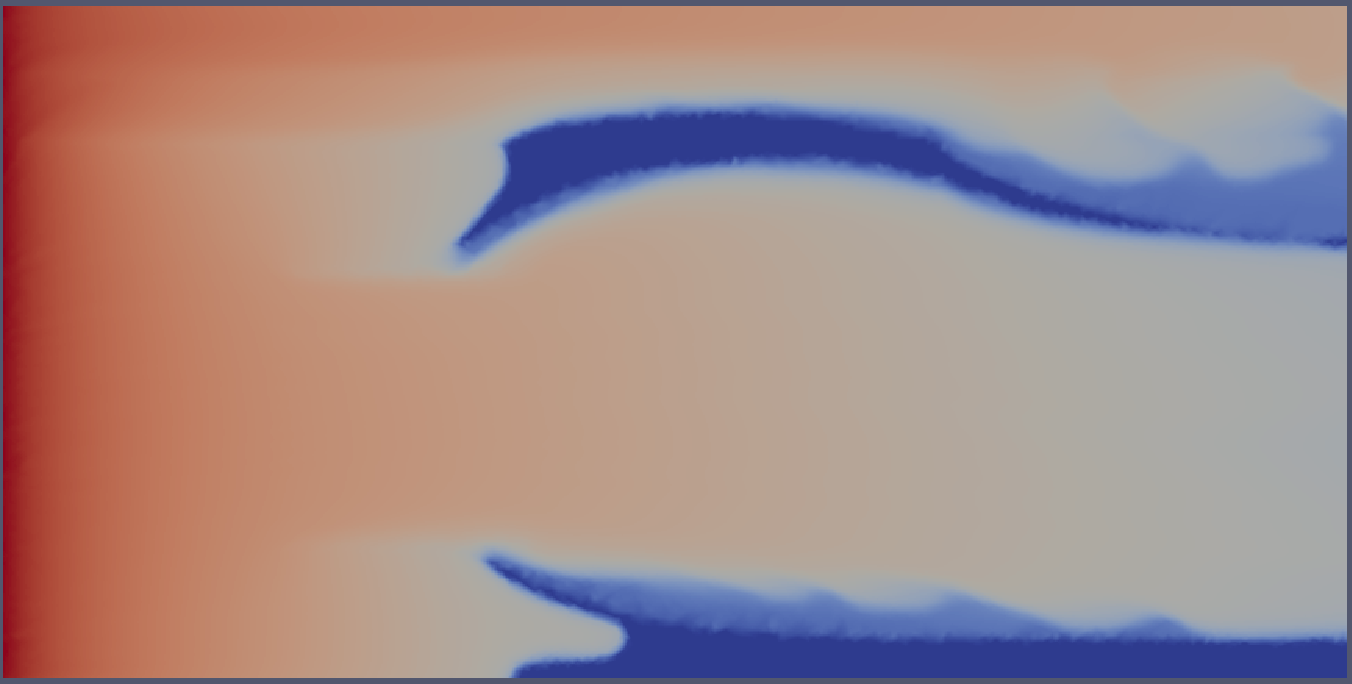
\includegraphics[width=.65\textwidth]{./Pics1/mr10_5regions_fixed/5regions_fixed_2000.pdf} 
}
\vspace{0.0cm}
\hbox{\hspace{6.5cm} (a) flow at t=end (fixed mesh)   
}
\vspace{0.25cm}
\hbox{\hspace{3.5cm}
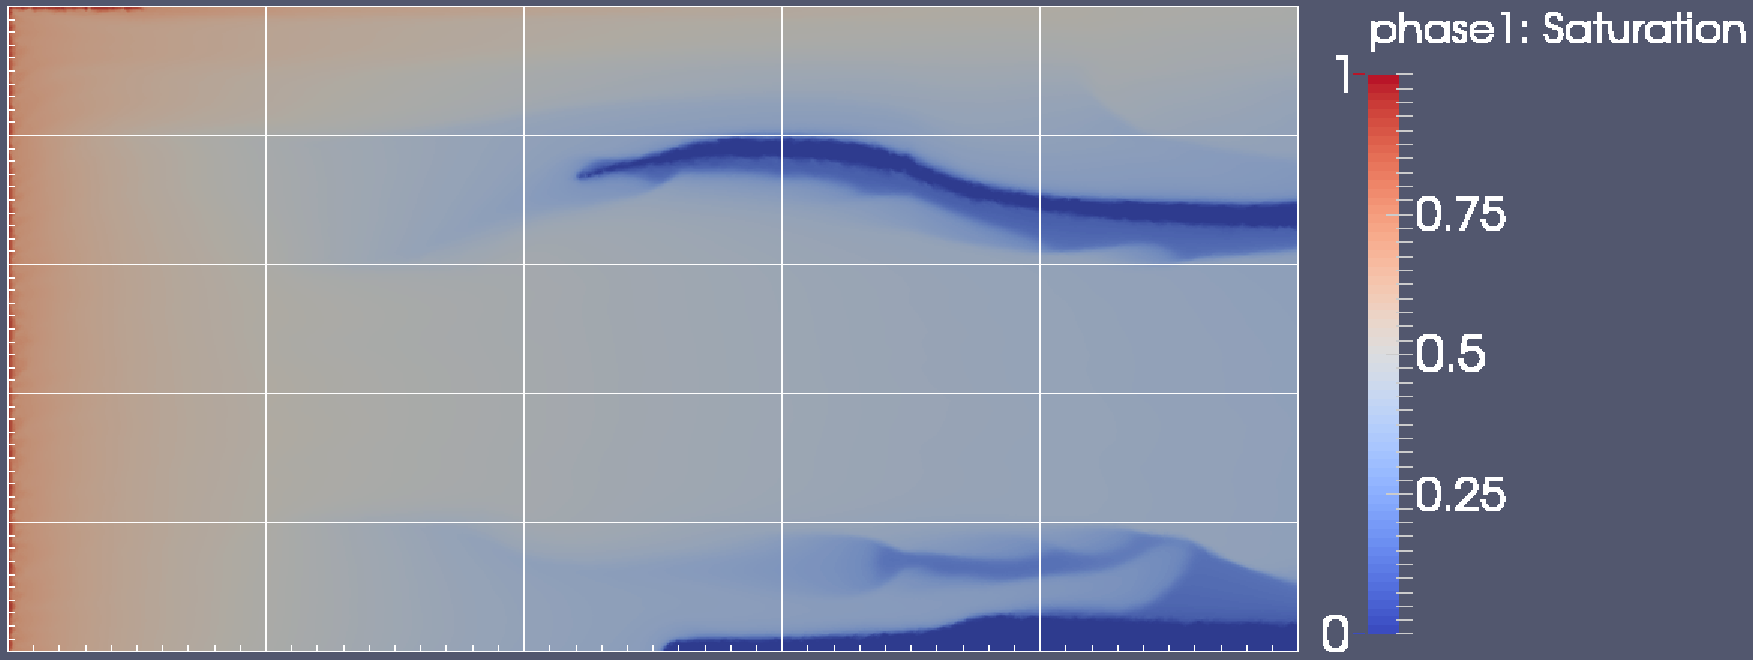
\includegraphics[width=.9\textwidth]{./Pics1/mr10_5regions_adapt/5regions_adapt_3000_1.pdf}
}
\vspace{0.0cm}
\hbox{\hspace{6.5cm} (b) flow at t=end (adaptive mesh)     
}
}     
\caption{Using the $P_{1}DGP_{2}$ element type for VR=$10$ under the same time steps, we compared the impact of fixed and adaptive mesh for the same timeframe. The end of simulation happens at $time=5 sec$ and for the timestemp $t=9999$ while the number of elements in both simulations was approximately $4700$. When adaptive mesh is introduce there is better repersentation of the fluid instabilities as these are developed on time.}
\label{fig:2testcase_d}
\end{figure}
\end{landscape}
\clearpage



%%%%
%%%%  FIGURE
%%%%
\begin{landscape}
\begin{figure}[ht] 
\vbox{
\hbox{\hspace{3.5cm}
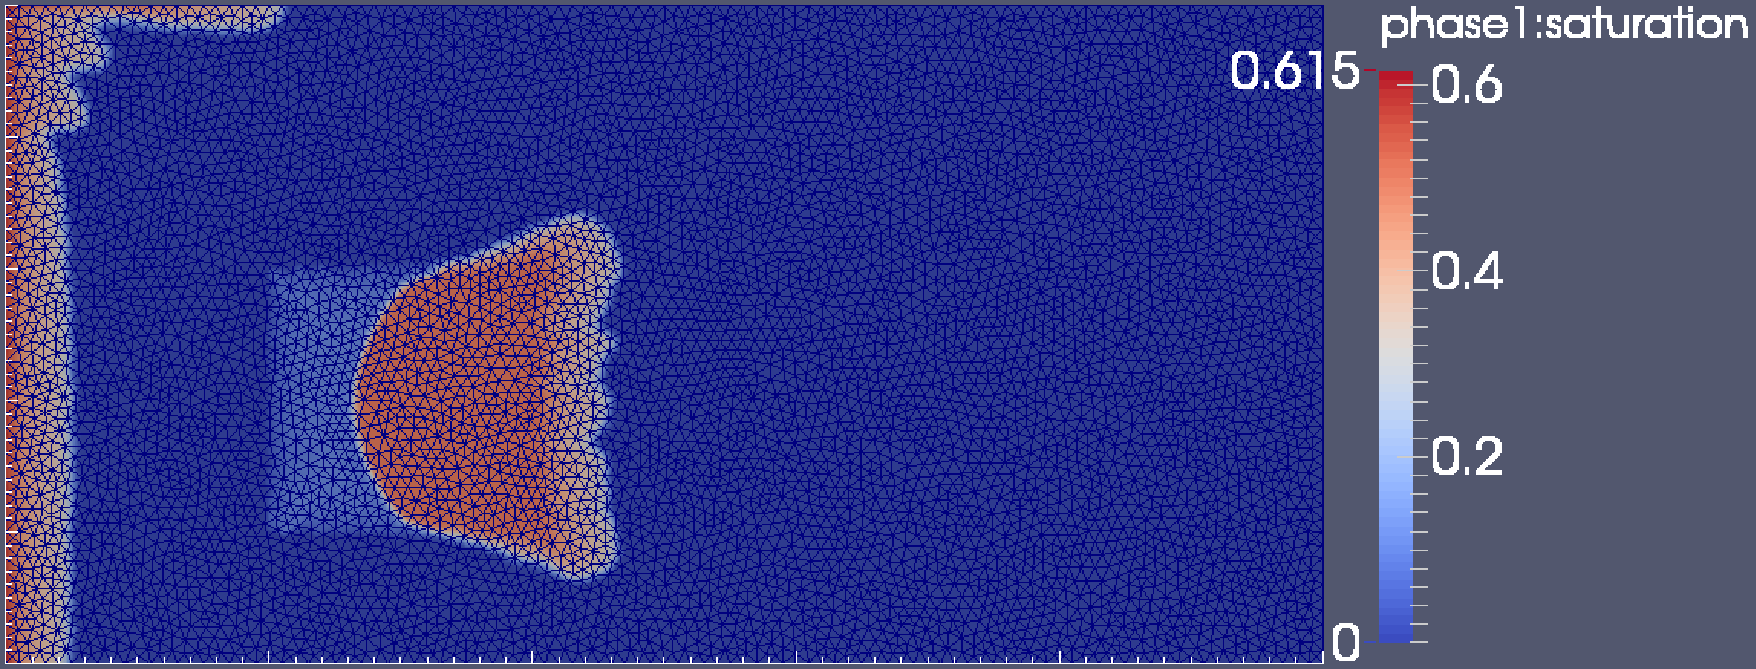
\includegraphics[width=.9\textwidth]{./Pics1/mr10_5regions_fixed_dinlet/5regions_dinlet_fixed_100_1.pdf}
}
\vspace{0.0cm}
\hbox{\hspace{6.5cm} (a) double inlet - fixed mesh   
}
\hbox{\hspace{3.5cm}
  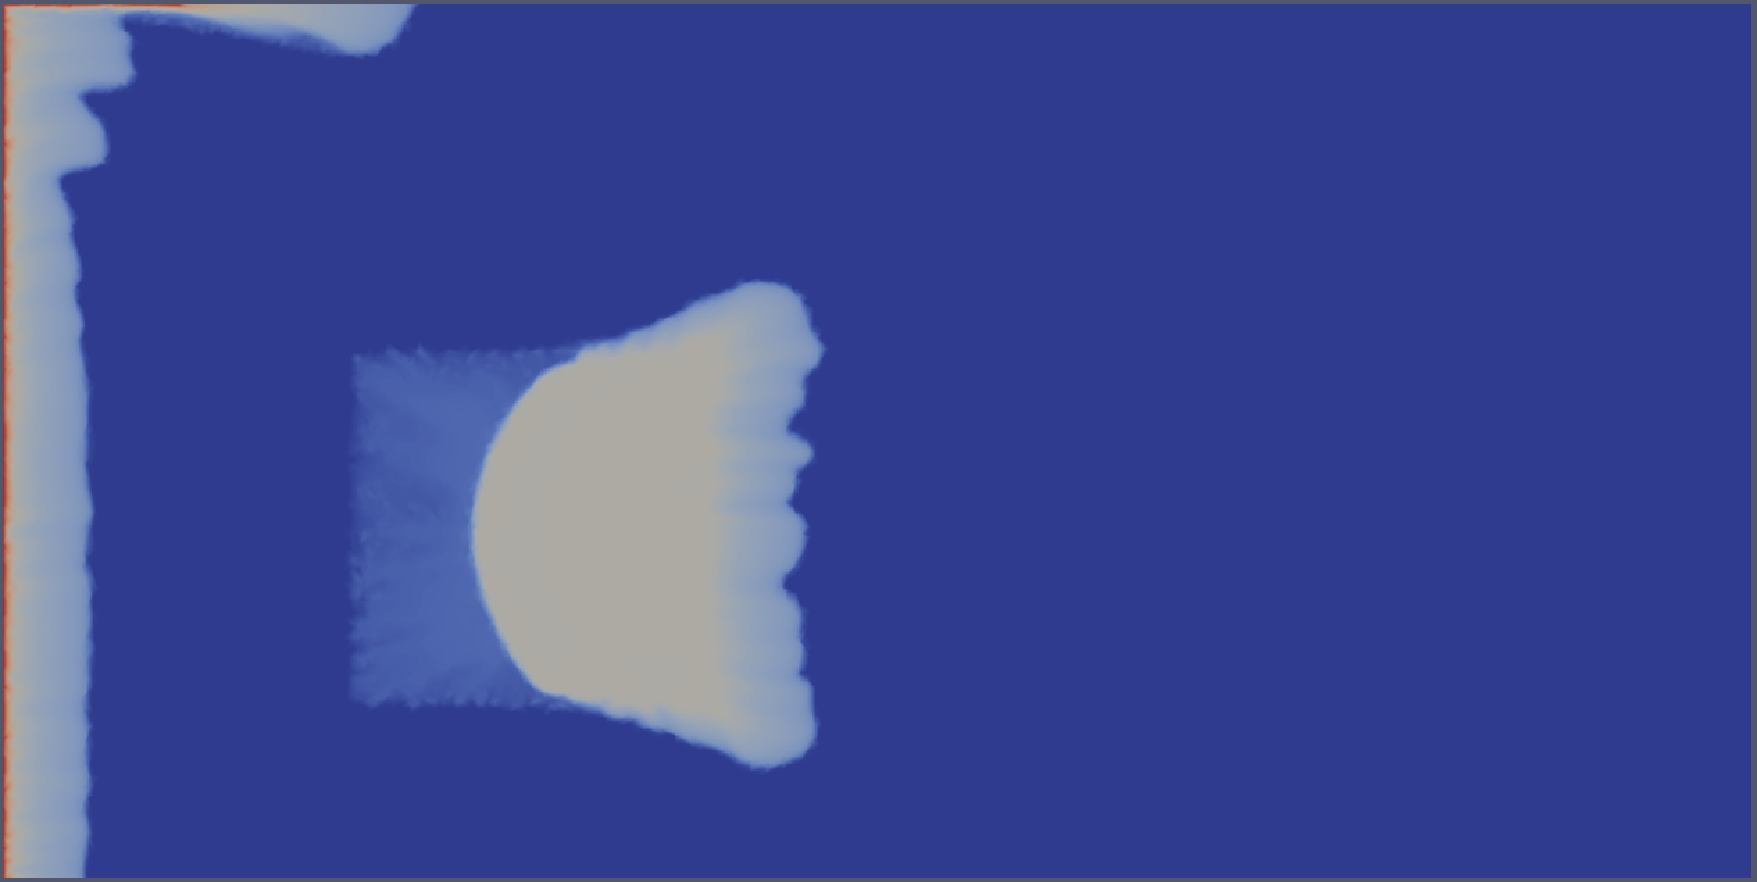
\includegraphics[width=.67\textwidth]{./Pics1/mr10_5regions_adapt_dinlet/5regions_dinlet_adapt_start.pdf}
}
\vspace{0.0cm}
\hbox{\hspace{6.5cm} (b) double inlet adaptive mesh   
}
}     
\caption{Comparing test-cases of fixed and adaptive mesh while a second region/inlet is introduced. For $t=0.101$s, using the $P_{1}DGP_{2}$ element type for MR=$10$ under the same time steps. For this simulation there are $13226$ elements for the fixed messh and $43716$ for the adaptive.}
\label{fig:3testcase_a}
\end{figure}
\end{landscape}
\clearpage

%%%%
%%%%  FIGURE
%%%%
\begin{figure}[ht] 
\vbox{
\hbox{\hspace{3.5cm}
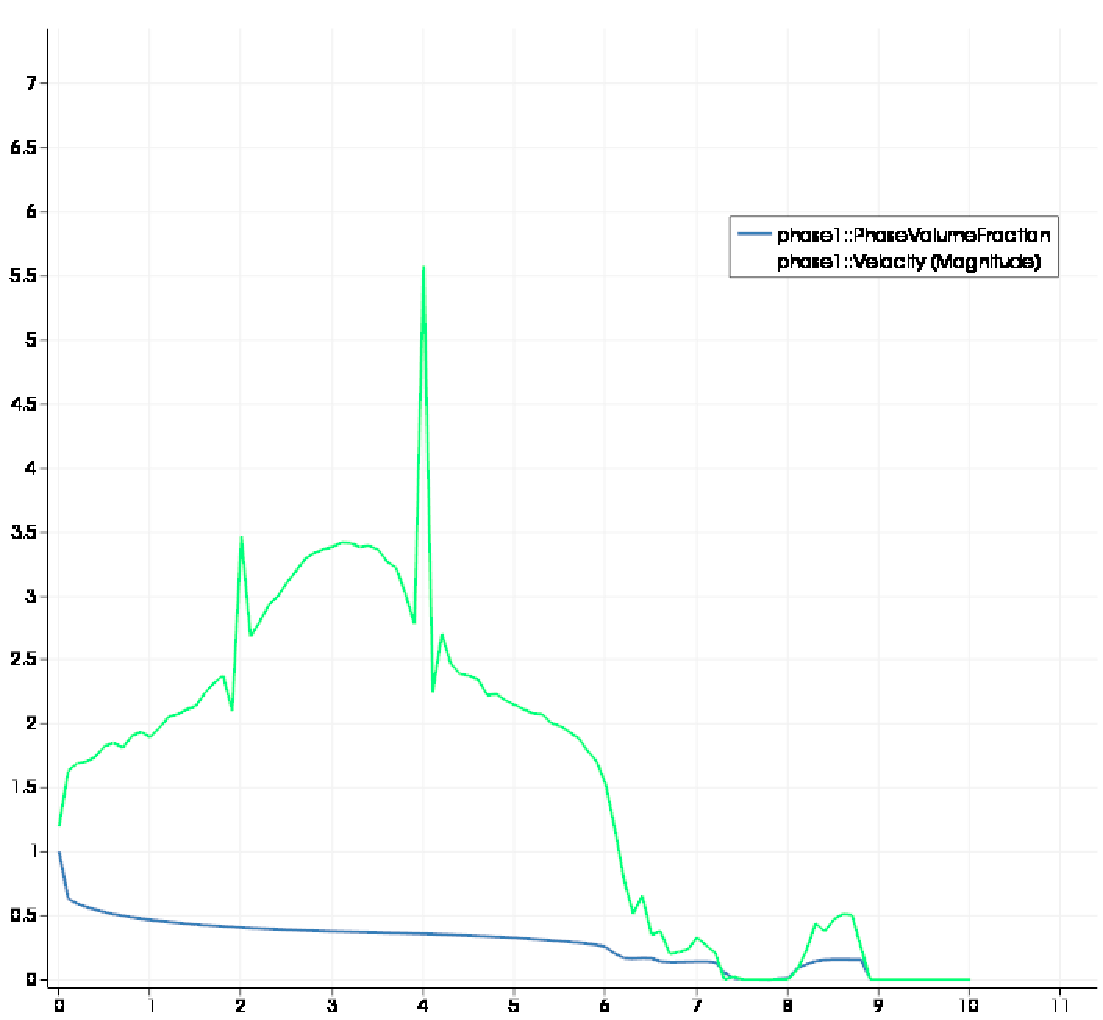
\includegraphics[width=.5\textwidth]{./Pics1/mr10_5regions_adapt/5regions_adapt_vel_magn.pdf} 
}
\vspace{0.0cm}
\hbox{\hspace{5.0cm} (a) single inlet velocity magnitude   
}
\hbox{\hspace{3.5cm}
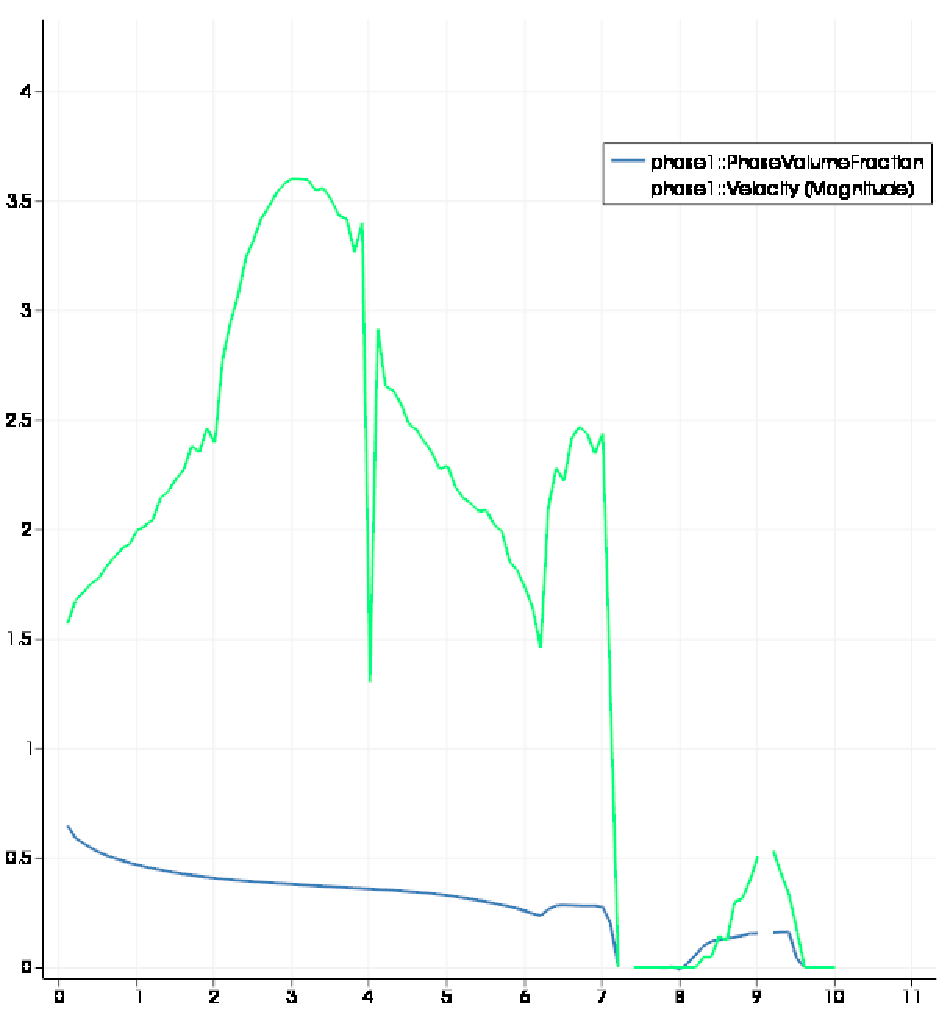
\includegraphics[width=.5\textwidth]{./Pics1/mr10_5regions_adapt_dinlet/5regions_dinlet_adapt_vel_magn.pdf}
}
\vspace{0.0cm}
\hbox{\hspace{5.0cm} (b) double inlet velocity magnitude   
}
}     
\caption{For the same time step, t=1000, these plots describe the velocity magnitudes of the phase $1$ (injected fluid) under the same boundary and initiall conditions. From top to bottom,these graphs describe the velocity magnitude %for fixed mesh is plotted(top), the velocity magnitude 
for adaptive mesh-single inlet (top) and the velocity magnitude for adaptive mesh with double inlet (bottom) as these are also presented in fig.\ref{fig:3testcase_a}. The main difference between the upper and lower plot %is not just the ability to capture in greater detail, the fluid instabilities as they happenduring the finger development and their velocity patterns. While there 
is the impact of the second injection interval as this can be seen from the slope and the rate that the velocity magnitude is changing.}
\label{fig:vel_magn}
\end{figure}

%%%%
%%%%  FIGURE
%%%%
\begin{landscape}
\begin{figure}[ht] 
\vbox{
\hbox{\hspace{3.5cm}
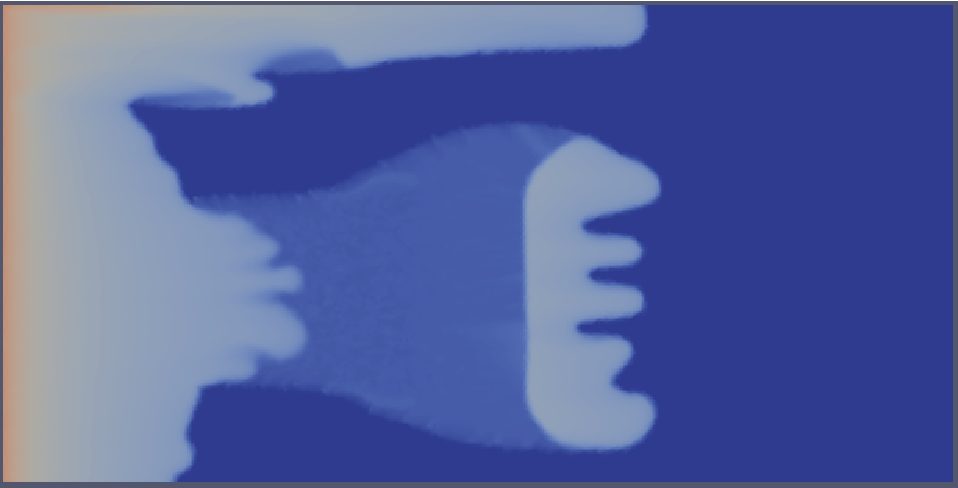
\includegraphics[width=.65\textwidth]{./Pics1/5reg_dinlet_fixed_500.pdf} 
}
\vspace{0.0cm}
\hbox{\hspace{6.5cm} (a) double inlet - fixed mesh   
}
\hbox{\hspace{3.5cm}
\includegraphics[width=.9\textwidth]{./Pics1/5reg_dinlet_adapt_500_1.pdf}
}
\vspace{0.0cm}
\hbox{\hspace{6.5cm} (b) double inlet adaptive mesh   
}
}     
\caption{For $t=5$s there is a comparison between fixed mesh(a) and adaptive mesh(b).}
\label{fig:3testcase_b}
\end{figure}
\end{landscape}
\clearpage

%%%%
%%%%  FIGURE
%%%%
\begin{landscape}
\begin{figure}[ht] 
\vbox{
\hbox{\hspace{3.5cm}
\includegraphics[width=.65\textwidth]{./Pics1/5reg_dinlet_fixed_1500.pdf} 
}
\vspace{0.0cm}
\hbox{\hspace{6.5cm} (a) double inlet - fixed mesh   
}
\hbox{\hspace{3.5cm}
\includegraphics[width=.9\textwidth]{./Pics1/5reg_dinlet_adapt_1500_1.pdf}
}
\vspace{0.0cm}
\hbox{\hspace{6.5cm} (b) double inlet adaptive mesh   
}
}     
\caption{For $t=7.5$s this is a comparison between fixed mesh(a) and adaptive mesh(b).}
\label{fig:3testcase_c}
\end{figure}
\end{landscape}
\clearpage

%%%%
%%%%  FIGURE
%%%%
\begin{landscape}
\begin{figure}[ht] 
\vbox{
\hbox{\hspace{3.5cm}
\includegraphics[width=.65\textwidth]{./Pics1/5reg_dinlet_fixed_end.pdf} 
}
\vspace{0.0cm}
\hbox{\hspace{6.5cm} (a) double inlet - fixed mesh   
}
\hbox{\hspace{3.5cm}
\includegraphics[width=.9\textwidth]{./Pics1/5reg_dinlet_adapt_end_1.pdf}
}
\vspace{0.0cm}
\hbox{\hspace{6.5cm} (b) double inlet adaptive mesh   
}
}     
\caption{This is a comparison between fixed mesh(a) and adaptive mesh(b) at the end of the simulation. For the fixed mesh at this point the maximum number of point is $13226$ while for the adaptive mesh is $7582$ and most of them are located where is needed in the domain.}
\label{fig:3testcase_d}
\end{figure}
\end{landscape}
\clearpage

%%%%
%%%%  FIGURE
%%%%
\begin{landscape}
\begin{figure}[ht] 
\vbox{
\hbox{\hspace{3.5cm}
\includegraphics[width=.8\textwidth]{./Pics1/mr100_fixed/mr100_fixed_500.pdf} 
}
\vspace{0.0cm}
\hbox{\hspace{4.0cm} (a) fixed and unstructured mesh for MR = 100 (start)   
}
\hbox{\hspace{3.5cm}
\includegraphics[width=.8\textwidth]{./Pics1/mr100_fixed/mr100_fixed_1500.pdf}
}
\vspace{0.0cm}
\hbox{\hspace{3.75cm} (b) fixed and unstructured mesh for MR = 100 (t = 1500)   
}
}     
\caption{For the case of VR=$100$ from top to bottom, the number of elements is $4680$ and fixed and unstructured mesh for the same time steps, t=$0.25$ or t=500(a), t=$0.75$ or t=1500(b). }
\label{fig:4testcase_a}
\end{figure}
\end{landscape}
\clearpage

%%%%
%%%%  FIGURE
%%%%
\begin{landscape}
\begin{figure}[ht] 
\vbox{
\hbox{\hspace{3.5cm}
\includegraphics[width=.8\textwidth]{./Pics1/mr100_fixed/mr100_fixed_3000.pdf} 
}
\vspace{0.0cm}
\hbox{\hspace{3.75cm} (c) fixed and unstructured mesh for MR = 100    
}
\hbox{\hspace{3.5cm}
\includegraphics[width=.8\textwidth]{./Pics1/mr100_fixed/mr100_fixed_end.pdf}
}
\vspace{0.0cm}
\hbox{\hspace{7.cm} (d) end of simulations     
}
}     
\caption{screenshot (c) is for t=$1.5$ sec or t=$3000$ and screenshot (d) is for t=$3.175$ sec, at the end of the simulations. }
\label{fig:4testcase_b}
\end{figure}
\end{landscape}
\clearpage





\end{document}

%%
%% End of tex file.
